% Built on the VLDB template (acmart with pvldb.sty), as the Hermes paper is.

\documentclass[sigconf, nonacm]{acmart}

\usepackage{pvldb}
% Packages and macros, following the conventions of the KROMA, MOIRA, and Hermes papers.
\usepackage{amsmath}
\usepackage{amssymb}
\usepackage{booktabs}
\usepackage{multirow}
\usepackage{xcolor}
\usepackage{xspace}
\usepackage{balance}
\usepackage{pgfplots}
\usepackage[ruled,linesnumbered,noend]{algorithm2e}
\pgfplotsset{compat=1.17}
\usetikzlibrary{positioning,arrows.meta}

% Long identifiers must not overflow the narrow columns.
\setlength{\emergencystretch}{2em}

% Tight layout, as in the MOIRA and Hermes papers: no stretched columns, small caption gaps,
% compact lists and floats. (acmart forbids titlesec.)
\raggedbottom
\usepackage[skip=0.5ex]{caption}
\setlength{\abovecaptionskip}{3pt}
\setlength{\belowcaptionskip}{3pt}
\usepackage{enumitem}
\setlist{nosep, leftmargin=*}
\setlength{\textfloatsep}{8pt plus 2pt minus 2pt}
\setlength{\floatsep}{6pt plus 2pt minus 2pt}
\setlength{\intextsep}{6pt plus 2pt minus 2pt}
\setlength{\dbltextfloatsep}{8pt plus 2pt minus 2pt}

\newcommand{\sys}{\textsc{OntoDB}\xspace}
\newcommand{\sparql}{SPARQL\xspace}
\newcommand{\kw}[1]{{\ensuremath{\mathsf{#1}}}\xspace}
\newcommand{\stitle}[1]{\vspace{1.2ex}\noindent{\bf #1}}
\newcommand{\ie}{\emph{i.e.,}\xspace}
\newcommand{\eg}{\emph{e.g.,}\xspace}
\newcommand{\desc}{\mathrm{desc}}
\newcommand{\po}{\mathit{po}}
\newcommand{\lo}{\mathit{lo}}
\newcommand{\ef}{\mathit{ef}}


\renewcommand\vldbdoi{XX.XX/XXX.XX}
\renewcommand\vldbpages{XXX-XXX}
\renewcommand\vldbavailabilityurl{https://github.com/lamng3/OntoDB}

\begin{document}

\title{OntoDB: A Fast Ontology Database for\\Pattern, Hierarchy, and Semantic Queries}

\author{Lam Nguyen}
\affiliation{%
  \institution{Case Western Reserve University}
  \city{Cleveland}
  \state{Ohio}
  \country{USA}
}
\email{ltn18@case.edu}

\begin{abstract}
Ontologies are queried in three ways: for the triples that match a pattern,
for the instances at or below a class, and for the terms closest in meaning
to a given term.
Triple stores answer the first well, handle the second by rewriting queries
or by materializing entailed triples, and leave the third to a separate
vector database; none is built to serve many threads from one embedded
engine, or to run in a web page.
We present \sys, an ontology database that answers all three kinds of query
inside one disk-based, multi-threaded engine.
Through \sys we make the following contributions.
(1) A B+ tree triple store of three permutations behind a buffer pool, with
algorithms for search, insert, delete, range scan, and bulk load, and a bound
on the pages a range scan reads.
(2) A concurrency design that scales: an optimistic leaf-only descent for
inserts and deletes, a sharded buffer pool whose hits take no latch, and a
one-word page latch.
(3) A labelling of the class hierarchy with postorder intervals kept in the
same B+ tree, so that ``everything under a class'' is a few range scans and no
entailed triple is stored.
(4) Exact, IVF, product-quantized, and HNSW vector indexes in the engine, a
proof that no linear order of points keeps neighbors close, and the finding
that in an ontology a class filter is correlated with the vectors, so the
usual independence assumption fails.
(5) A 0.85\,MB WebAssembly build that runs the engine in a browser.
On LUBM and the Gene Ontology, against Oxigraph, Apache Jena TDB2, and SQLite,
\sys answers selective triple patterns 3 to 37$\times$ faster and the
instances of a class 2 to 48$\times$ faster, and serves 3 to 7$\times$ more
lookups per second with eight threads (1.46 million per second).
Its interval labels store 8.1$\times$ fewer triples than materializing the
hierarchy and read 48$\times$ fewer pages than rewriting the query, and exact
pre-filtering through them is $10^2$ to $10^4\times$ faster than any index
strategy for classes below about 1,000 members.
\end{abstract}


\keywords{ontology, triple store, B+ tree, RDFS, vector search, WebAssembly}

\maketitle

\vldbtopmatter

\section{Introduction}
\label{sec-intro}

Ontologies such as the Gene Ontology~\cite{ashburner2000} and the schemas of
enterprise knowledge graphs are stored as sets of triples and queried in
three ways.
A \emph{pattern} query asks for the triples that match a template, such as
the resources of one type, and is the base case of every RDF
store~\cite{weiss2008,neumann2010}.
A \emph{structural} query asks for the instances at or below a class, and
needs the class hierarchy.
A \emph{semantic} query asks for the terms closest in meaning to a given
term, which has no answer in the data and needs a similarity measure over
embeddings.
The three meet in queries such as ``the terms most similar to
\emph{apoptotic process} that lie under \emph{cell death}''.

Existing systems leave four problems open.
\textbf{C1. Hierarchy costs space or time.}
RDFS entailment is either \emph{materialized} at write time, which stores
every inferred triple~\cite{rdfox}, or \emph{rewritten} into the query,
which scans once per subclass.
On the Gene Ontology with 200,000 typed entities, materializing the closure
multiplies the triples by 8.1, and rewriting reads 48 times more pages than
a store that knows the hierarchy.
\textbf{C2. A sorted index does not hold meaning.}
Triple stores answer patterns with range scans over sorted permutations.
It is tempting to believe that neighbors in meaning are neighbors in the
order; we prove they cannot all be (Section~\ref{sec-order}), and measure how
few are.
Similarity is therefore left to a vector database next to the triple store,
with its own storage, its own paging, and no view of the hierarchy.
\textbf{C3. A class filter is correlated with the vectors.}
Filtered vector search is usually costed by assuming that the filter is
independent of the similarity.
In an ontology it is not: the neighbors of a term lie under the term's own
ancestors.
A post-filtered index can then find 7\% of the right answers, and the
independence estimate of the work it must do is wrong in both directions
(Section~\ref{sec-vectors}).
\textbf{C4. A paged store must scale across threads.}
A classic buffer pool serializes every page access on one latch, and a
classic B+ tree write latches the root.
In our first version, lookups per second fell from 330 thousand with one
thread to 180 thousand with eight, and inserts from 184 thousand to 23
thousand: a store embedded in a service or a notebook that answers many
queries at once spent its time waiting for itself.

\begin{example}
\label{exa-motivation}
Let $q$ be the term \emph{apoptotic process} in the Gene Ontology and $c$ the
class \emph{cell death}.
The query asks for the five terms nearest to $q$ in embedding space among
the 97 classes at or below $c$ in an 834-class slice of the ontology.
A triple store alone cannot rank by meaning.
A vector index alone returns neighbors from anywhere in the ontology, and
a post-filter keeps those under $c$ only if enough of them are.
\sys finds the 97 classes with one range scan of the same B+ tree that holds
the triples, scores them exactly, and returns \emph{apoptotic process
involved in development} (cosine 0.865) first, in under a millisecond in a
web page.
\end{example}

Database systems have handled a similar split for decades: an access method
is added to the engine that owns the storage, paging, and logging, and not
beside it.
This paper takes that view of ontologies.

\stitle{Contributions}.
This paper introduces \sys, an open-source ontology database in C++20
(Figure~\ref{fig-arch}), with five technical contributions.
\begin{enumerate}
\item \textbf{A concurrent B+ tree triple store} (Sections~\ref{sec-store}
  and~\ref{sec-conc}). Three permutations behind a buffer pool, with the
  algorithms for search, insert, and delete, a bound on the pages a range scan
  reads, and a latch-free hit path and an optimistic writer descent that scale
  to eight threads.
\item \textbf{Hierarchies as intervals} (Section~\ref{sec-labels}). A
  postorder labelling of the class DAG kept in the same B+ tree, so that
  ``everything under $c$'' is a few range scans and no entailed triple is
  stored.
\item \textbf{An entailment-aware plan rewrite} (Section~\ref{sec-rewrite}).
  RDFS subclass entailment of \texttt{rdf:type} patterns as interval scans the
  optimizer costs and joins like any other, with the answers of
  materialization, prepared 16 times faster and in 8 times less space.
\item \textbf{Vector indexes and filtered search}
  (Sections~\ref{sec-order} and~\ref{sec-vectors}). A proof that no sorted
  order keeps neighbors close, IVF posting lists stored as key ranges of the
  triple tree, and the finding that a class filter is correlated with
  similarity, with the rule that chooses between pre-filtering and masked
  search.
\item \textbf{A build for the browser} (Section~\ref{sec-system}). The whole
  engine, with its paged trees and semantic search, as a 0.85\,MB WebAssembly
  module.
\end{enumerate}
We evaluate \sys against Oxigraph~\cite{oxigraph}, Apache Jena
TDB2~\cite{jenatdb}, and SQLite on LUBM~\cite{lubm} and the Gene Ontology
(Section~\ref{sec-exp}, summarized in Table~\ref{tab-glance}).
The code, data generators, and benchmark programs are available at the
artifact URL above.

\section{Preliminaries}
\label{sec-pre}

\begin{table}[t]
\caption{Notation.}
\label{tab-notation}
\small
\begin{tabular}{@{}p{2.15cm}p{5.6cm}@{}}
\toprule
Symbol & Meaning \\
\midrule
$(s,p,o)$, $\mathcal{T}$, $n$ & a triple; the set of triples; $n=|\mathcal{T}|$ \\
$\mathit{id}(a)$ & dictionary id of term $a$ \\
$x$, $\sigma$ & a B+ tree key, three ids in 24 bytes; a separator key \\
$e$ & an instance (an entity with a type) \\
$\pi$, $\ell(\pi)$ & a permutation (SPO, POS, OSP); the length of the prefix of $\pi$ a pattern binds \\
$B$, $F$ & capacity of a leaf (169 keys) and of an internal page (144 separators) \\
$h$ & height of a B+ tree \\
$P$, $Q$, $R$ & a page; its parent; its right sibling \\
$[a,b)$, $r$ & a half-open key range; the number of keys a scan returns \\
$H=(\mathcal{C},E)$ & the class hierarchy, a DAG of classes $\mathcal{C}$ and subclass edges $E$ \\
$\desc(c)$ & the classes at or below $c$, including $c$ \\
$\po(c)$, $\lo(c)$ & postorder number of $c$; smallest number in its subtree of the spanning forest \\
$I(c)$ & the set of intervals that covers the numbers of $\desc(c)$ \\
$E'(c)$ & non-tree edges whose tail is in $\desc(c)$ \\
$f(c)$ & fraction of terms in $\desc(c)$: $|\desc(c)|/N$ \\
$N$, $d$ & number of terms with vectors; vector dimension \\
$\mathbf{v}(t)$, $\mathrm{sim}$ & unit vector of $t$; cosine similarity \\
$q$, $k$ & the query term; the number of neighbors asked for \\
$\mathrm{inst}(c)$, $\mathrm{near}(q,c,k)$ & the instance query and the filtered similarity query \\
$\nu$, $\rho$ & IVF: number of lists; lists probed per query \\
$S$, $\tau$ & buffer-pool shards; threads \\
$m$ & product quantization: pieces per vector \\
$M$, $\ef$ & HNSW: links per node; search beam width \\
$G$, $D$ & a graph and its diameter (Lemma~\ref{lem-bw}) \\
\bottomrule
\end{tabular}
\end{table}

\stitle{Triples and patterns}.
An RDF graph is a set $\mathcal{T}$ of triples $(s,p,o)$ of subject,
predicate, and object, with $n=|\mathcal{T}|$.
A \emph{triple pattern} $(s,p,o)$ replaces some positions by variables,
written $\cdot$ here when the variable is not used elsewhere; its answers
are the triples of $\mathcal{T}$ that agree with it on every bound position.
A \emph{basic graph pattern} is a set of triple patterns joined on shared
variables.
Following common practice~\cite{weiss2008,neumann2010}, \sys replaces each
term $a$ by a dense integer $\mathit{id}(a)$ and stores triples as
three-integer keys.

\stitle{Class hierarchy}.
The \texttt{rdfs:subClassOf} triples define a directed graph
$H=(\mathcal{C},E)$ over classes, with an edge $(c,c')$ when $c$ is a
subclass of $c'$.
We write $\desc(c)$ for the classes at or below $c$, including $c$ itself, and
call a class \emph{below} $c$ when it is in $\desc(c)$.
Cycles are collapsed into one class, since the classes on a cycle are
equivalent.
The \emph{instances} of $c$ are the subjects $e$ with a triple
$(e,\texttt{rdf:type},c')$ for some $c'\in\desc(c)$.

\stitle{Similarity}.
Each term $t$ among $N$ terms has a unit vector $\mathbf{v}(t)\in\mathbb{R}^d$
produced by an embedding model, and the similarity of two terms is the cosine
$\mathrm{sim}(t,u)=\mathbf{v}(t)\cdot\mathbf{v}(u)$.

\begin{definition}[Queries]
\label{def-queries}
Given the data above, \sys answers
(i) a \emph{pattern query}, the answers of a basic graph pattern;
(ii) an \emph{instance query} $\mathrm{inst}(c)$, the instances of a class
$c$; and
(iii) a \emph{filtered similarity query} $\mathrm{near}(q,c,k)$, the $k$
terms $t\in\desc(c)$, $t\ne q$, that maximize $\mathrm{sim}(q,t)$.
\end{definition}

\noindent
Table~\ref{tab-notation} lists the notation used throughout.


\section{The OntoDB Store}
\label{sec-store}

\sys is a single-process engine with the layers of a conventional disk-based
DBMS (Figure~\ref{fig-arch}).
A \sparql query is parsed, bound against the dictionary, planned as a
left-deep tree, reordered by the optimizer, and run by volcano-style
executors that pull rows of term ids.
The executors read triples through a store interface.
The \emph{indexed store}, which this paper is about, keeps each triple in
three B+ trees in one page file, behind a buffer pool with LRU-K
eviction~\cite{oneil1993}; terms are encoded by a dictionary built from the
same parts, a heap of spellings and two B+ trees.
Updates are logged page by page for ARIES-style recovery~\cite{mohan1992}.
The semantic extension of Sections~\ref{sec-labels} and~\ref{sec-vectors}
sits beside the store and reads it through the same interface.

\begin{figure}[t]
\centering
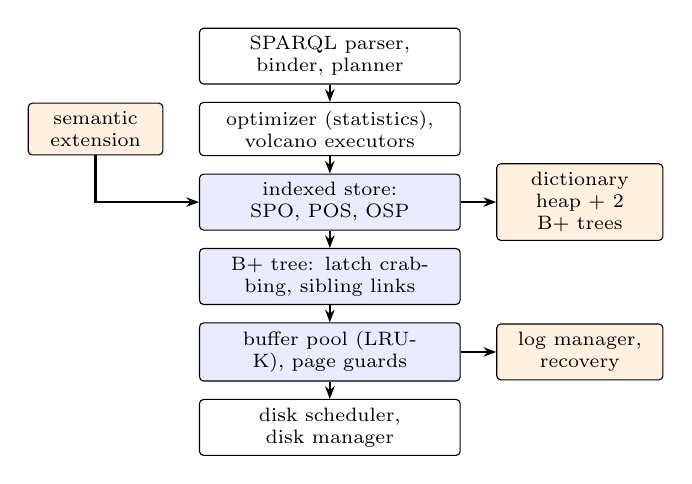
\begin{tikzpicture}[font=\scriptsize,
  box/.style={draw,rounded corners=1.5pt,minimum height=0.55cm,inner sep=3pt,align=center,fill=white,text width=3.1cm},
  side/.style={draw,rounded corners=1.5pt,minimum height=0.55cm,inner sep=3pt,align=center,fill=orange!12,text width=1.9cm},
  arr/.style={-{Stealth[length=1.6mm]},thick}]
\node[box] (q) {\sparql parser, binder, planner};
\node[box,below=0.22cm of q] (o) {optimizer (statistics), volcano executors};
\node[box,below=0.22cm of o,fill=blue!8] (s) {indexed store: SPO, POS, OSP};
\node[box,below=0.22cm of s,fill=blue!8] (t) {B+ tree: latch crabbing, sibling links};
\node[box,below=0.22cm of t,fill=blue!8] (b) {buffer pool (LRU-K), page guards};
\node[box,below=0.22cm of b] (d) {disk scheduler, disk manager};
\node[side,right=0.45cm of s] (dict) {dictionary\\heap + 2 B+ trees};
\node[side,right=0.45cm of b] (log) {log manager,\\recovery};
\node[side,left=0.45cm of o,text width=1.5cm] (sem) {semantic\\extension};
\draw[arr] (q) -- (o); \draw[arr] (o) -- (s); \draw[arr] (s) -- (t); \draw[arr] (t) -- (b); \draw[arr] (b) -- (d);
\draw[arr] (s) -- (dict); \draw[arr] (b) -- (log);
\draw[arr] (sem) |- (s);
\end{tikzpicture}
\caption{The layers of \sys. Blue boxes are the storage structures of Section~\ref{sec-store}.}
\label{fig-arch}
\end{figure}

\subsection{Keys, Pages, and Permutations}

A triple is a 24-byte key $x$ of three dictionary ids, stored big-endian so that
\texttt{memcmp} is the order.
A page is 4\,KiB; a leaf holds up to $B{=}169$ keys and an internal page up
to $F{=}144$ separators with $F{+}1$ child ids.
Leaves are linked to their \emph{right} sibling only.
A header page names the root, so a root split changes one word.
Every page but the root keeps at least half its maximum: a leaf at least
$\lfloor B/2\rfloor=84$ keys, an internal page at least
$\lfloor F/2\rfloor{+}1=73$ children.

Three permutations are enough.
A pattern binds some of $s$, $p$, $o$, and with the permutations SPO, POS,
and OSP every pattern has one in which its bound positions form a prefix
(Table~\ref{tab-perms}); it is then one range scan that returns only
matching triples.
Algorithm~\ref{alg-pattern} (Appendix~\ref{apx-alg}) picks the permutation with the longest bound
prefix.
The other three permutations would make no pattern cheaper
(Section~\ref{sec-exp}).

\begin{table}[t]
\caption{The permutation $\pi$ that answers each pattern, and the length $\ell(\pi)$ of the bound prefix.}
\label{tab-perms}
\small
\resizebox{\columnwidth}{!}{%
\begin{tabular}{@{}lccccccc@{}}
\toprule
Pattern & $(s,\cdot,\cdot)$ & $(\cdot,p,\cdot)$ & $(\cdot,\cdot,o)$ & $(s,p,\cdot)$ & $(\cdot,p,o)$ & $(s,\cdot,o)$ & $(s,p,o)$ \\
$\pi$, $\ell(\pi)$ & SPO, 1 & POS, 1 & OSP, 1 & SPO, 2 & POS, 2 & OSP, 2 & SPO, 3 \\
\bottomrule
\end{tabular}}
\end{table}


\subsection{Search}

A point lookup and the start of every scan use one descent.
\textsc{ChildFor} picks the child whose range holds $x$: the last separator
that is $\le x$, or child 0 if none is.
The descent \emph{crabs}: it latches the child before it releases the parent,
so a concurrent split cannot move $x$ away between two
steps~\cite{lehman1981,graefe2011}.

\begin{algorithm}[t]
\caption{\textsc{LeafFor}$(x)$ and \textsc{Contains}$(x)$}\label{alg-search}
\small
latch the header page (shared); $P \gets$ the root; \lIf{$P$ is nil}{\Return nil}
latch $P$ (shared); release the header\;
\While{$P$ is an internal page}{
  $P' \gets \textsc{ChildFor}(P,x)$ \tcp*{binary search over the separators}
  latch $P'$ (shared); release $P$; $P \gets P'$\;
}
\Return $P$\;
\medskip
\textsc{Contains}$(x)$: $P \gets \textsc{LeafFor}(x)$; \Return whether $x$ is in $P$ (binary search)\;
\end{algorithm}

A lookup reads $h$ pages.
Every non-root leaf holds at least 84 keys and every non-root internal page
has at least 73 children, so a tree of $n$ keys has at most $n/84$ leaves
and height $h \le 2 + \log_{73}(n/84)$: at most four levels for the 1.3
million triples of LUBM(10), and three when the tree is bulk-loaded (about
7,800 full leaves under 54 internal pages).

\subsection{Insert}

Insert is \emph{pessimistic} crabbing.
It latches the header and then each page on the way down in write mode, and
releases every latched ancestor, the header included, as soon as the page
just latched is \emph{safe}, meaning it cannot split.
What is still latched at the leaf is exactly what a split can reach, so a
split never needs a latch it does not hold, and latches are taken in one
order everywhere: the header, then top to bottom, siblings left to right.

\begin{algorithm}[t]
\caption{\textsc{Insert}$(x)$}\label{alg-insert}
\small
latch the header (exclusive); \lIf{the tree is empty}{make a leaf holding $x$ the root; \Return true}
$\mathit{path} \gets [\,]$; $P \gets$ the root\;
\Repeat{$P$ is a leaf}{
  latch $P$ (exclusive)\;
  \If{$P$ is not full}{release every latch in $\mathit{path}$ and the header \tcp*{$P$ is safe}}
  push $P$ on $\mathit{path}$; $P \gets \textsc{ChildFor}(P,x)$\;
}
$P \gets \mathit{path}.\text{pop}()$; \lIf{$x \in P$}{\Return false}
insert $x$ into $P$; \lIf{$|P| \le B$}{\Return true}
\tcp{split the leaf: the left half stays, the right half moves, its first key is \emph{copied} up}
$R \gets$ new leaf with the upper half of $P$; $R.\text{next} \gets P.\text{next}$; $P.\text{next} \gets R$; $\sigma \gets R.\text{keys}[0]$\;
\While{true}{
  \If{$\mathit{path}$ is empty}{make a new root over $(P, R)$ with separator $\sigma$; set it in the header; \Return true}
  $Q \gets \mathit{path}.\text{pop}()$; insert $(\sigma, R)$ into $Q$ after $P$\;
  \lIf{$Q$ has at most $F$ separators}{\Return true}
  \tcp{split the internal page: the middle separator \emph{moves} up and leaves both halves}
  $P \gets Q$; $R \gets$ new page with the upper half of $Q$; $\sigma \gets$ the middle separator of $Q$\;
}
\end{algorithm}

A leaf split leaves two leaves of $\lfloor (B{+}1)/2\rfloor$ and
$\lceil (B{+}1)/2\rceil$ keys, so the half-full invariant holds.
Splits propagate only while the parent is full, so with random keys a split
costs $O(1/B)$ page writes per insert on average.
A split or a merge is the only update that spans pages, and
Section~\ref{sec-store-log} makes it atomic for recovery.

\subsection{Delete}

Delete crabs the same way with a different notion of safe: a page above its
minimum (for the root, more than one key), because only then can it not
underflow.
After removing $x$, a leaf below $\lfloor B/2\rfloor$ keys repairs itself
against a sibling under the same parent, preferring the left one.

\begin{algorithm}[t]
\caption{\textsc{Remove}$(x)$}\label{alg-remove}
\small
descend as in \textsc{Insert}, releasing ancestors when the page just latched is safe (above its minimum)\;
$P \gets$ the leaf; \lIf{$x \notin P$}{\Return false}
remove $x$ from $P$; \lIf{$P$ is the root or $|P| \ge \lfloor B/2\rfloor$}{\Return true}
\While{the page $P$ on top of $\mathit{path}$ is under its minimum and has a parent $Q$}{
  $R \gets$ the left sibling of $P$ under $Q$ (the right one if $P$ is first); latch siblings left to right\;
  \eIf{the entries of $P$ and $R$ fit in one page}{
    \textbf{merge}: move the right page's entries into the left (a leaf keeps its sibling link; an internal page pulls the separator down); delete the right entry from $Q$\;
  }{
    \textbf{redistribute}: move one entry from $R$ to $P$ (a leaf moves a key; an internal page rotates through $Q$) and fix the separator in $Q$\;
  }
  $P \gets Q$\;
}
\lIf{the root has one child left}{make the child the root and free the old root}
\end{algorithm}

A leaf emptied by a merge is \emph{kept}, empty, with its sibling link still
pointing on, rather than freed.
An iterator may already hold its id (next subsection), and an empty page it
can step through is cheaper than a protocol that tells every iterator the
page is gone.
Space reclaimed this way is not reused until the tree is rebuilt; freed
internal pages are unreachable once their parent is updated and are
released.

\subsection{Range Scan}

The half-open range $[a,b)$ is the primitive the semantic extension needs
(Section~\ref{sec-labels}); a prefix scan is a range between the smallest and
the largest key with that prefix.
\textsc{BeginRange} descends to the leaf for $a$, finds the first key
$\ge a$ by binary search, and hands the leaf to an iterator.


The iterator \emph{copies} the keys of a leaf that lie below $b$, remembers
the right sibling's id, and releases the leaf.
It holds no latch and no pin between rows, so a consumer that stalls, such as
a join waiting on its other input or a client reading slowly, blocks no
writer and pins no frame.
Reading the next leaf is one page read and no descent.
The cost is the copy and a weaker guarantee: between two leaves a writer may
change the tree, so a scan sees each leaf as it was when it was read, and
the transaction layer's locks, not the latches, give a query its isolation.
The iterator checks that keys increase along the chain and that a run of
empty leaves does not cycle, and stops with an error otherwise.

\begin{lemma}[Cost of a range scan]\label{lem-scan}
A scan that returns $r$ keys from an insert-only or bulk-loaded tree of
height $h$ reads at most $h + \lceil r/\lfloor B/2\rfloor\rceil$ pages, and at
most $h + \lceil r/B\rceil$ in a bulk-loaded tree.
\end{lemma}
\begin{proof}
The descent ends at the first leaf, which is one of the $h$ pages.
Every leaf after it holds at least $\lfloor B/2\rfloor$ keys, all inside the
range except possibly the last, so at most $\lceil r/\lfloor
B/2\rfloor\rceil$ more leaves are read.
A bulk-loaded leaf is full, which replaces $\lfloor B/2\rfloor$ by $B$.
\end{proof}

\subsection{Bulk Load}

Loading a file inserts hundreds of thousands of triples into an empty store,
and inserting one at a time leaves leaves about half full.
\sys instead sorts the triples once for each permutation and builds the tree
bottom-up.


Each page is written once, in order, and no page is split.
A bulk-loaded tree is full, which Section~\ref{sec-exp} measures.

\subsection{Buffer Pool, Dictionary, and Query Processing}

\stitle{Buffer pool}.
Pages live in a fixed set of frames.
A \emph{page guard} pins a frame and takes its latch for the guard's
lifetime, and its destructor releases both, so no path leaves a page pinned.
A frame is evicted by LRU-K with $K{=}2$~\cite{oneil1993}, which ranks a
frame by the time of its second most recent use and so is not flooded by one
long scan.
Reads and writes go through a disk scheduler.

\stitle{Dictionary}.
Terms (IRIs, literals with a language or datatype, blank nodes) have one
canonical spelling and get a dense 64-bit id in the order they first appear.
The mapping is stored in pages: spellings in a heap, \emph{id $\to$ record}
in a B+ tree keyed (id, page, slot), and \emph{spelling $\to$ id} in a B+
tree keyed (hash, id) with a 64-bit FNV-1a hash; a lookup scans the hash
prefix and compares the candidates' spellings, so a collision costs a
comparison and not a wrong answer.
Decoding an id costs a tree descent and a heap read, about $0.7\,\mu$s, and
a query that returns thousands of rows decodes thousands of ids.
A direct-mapped cache of the 65,536 most recently decoded spellings (slot
$=$ id mod size) removes most of that on a warm store; ids are dense and a
spelling never changes, so an entry is never stale.
Section~\ref{sec-exp} says where the cache helps and where it does not.

\stitle{Planning and joins}.
The planner builds a left-deep tree of triple scans in textual order and the
optimizer reorders it greedily: it appends, at each step, a pattern that
shares a variable with what is already joined (any pattern, if none does),
the one whose estimated join output is smallest.
The output of a join of inputs of $a_1$ and $a_2$ rows is estimated as
$a_1a_2/\max(V_1,V_2)$, where $V_1$ and $V_2$ are the numbers of distinct values
of the join variable, from exact counts that the store
collects at load for every position, every pair of positions, and every
triple.
The join operator is a nested loop, an index nested loop (the inner scan is
reopened with the outer row's bindings as constants, so it is again a prefix
scan of one tree), or a hash join, chosen per node.
The \sparql subset is basic graph patterns with \texttt{FILTER},
\texttt{DISTINCT}, \texttt{ORDER BY}, \texttt{LIMIT}, \texttt{OFFSET}, and
\texttt{INSERT DATA} and \texttt{DELETE DATA}; \texttt{OPTIONAL},
\texttt{UNION}, property paths, and aggregates are not implemented.

\subsection{Transactions and Recovery}
\label{sec-store-log}

Updates run under strict two-phase locking with a deadlock detector.
Recovery is page-oriented: when a dirty page is released, the pool appends a
record holding the page's image and stamps the page with its log sequence
number, and before a page is written the pool forces the log to that stamp.
Redo therefore copies page images whose stamp is older than the record and
needs no knowledge of the B+ tree layout.
Undo of a triple is \emph{logical} and writes a compensation record, because
other transactions may have changed the page since.
A split or merge is the one update that spans pages: insert and remove open a
\emph{page group} that holds the log back from the group's first record
until it ends, and the pool does not choose a page of the group as a victim,
so a crash never leaves half a split on disk.
Commit forces the log, and checkpoints are sharp (flush every page, then
write the record).
A crash harness kills the process between the pages of every multi-page
operation and checks the tree afterwards: sorted keys, separators consistent
with leaves, a leaf chain that visits every key once, and the half-full
bound.

\section{Concurrency}
\label{sec-conc}

An ontology store embedded in a service answers many queries at once while
facts arrive.
Strict two-phase locking keeps transactions isolated (Section~\ref{sec-store-log});
this section is about the \emph{latches} that keep the pages and the trees
sound, which decide how many threads the engine can use.
Our first implementation followed the textbook: one latch over the buffer
pool's tables, a mutex over the dictionary, and a root-to-leaf chain of
exclusive latches for every insert.
Sampling a run of eight reader threads showed that four of five samples were
threads waiting for a lock: 80\% of the waits were on the pool's latch and
20\% on the dictionary's mutex.
Once those were gone the next waits were on the shard latch of the pages every
query touches and on the page latches themselves (a \texttt{shared\_mutex} keeps
its reader count behind an internal mutex, so readers of one root page queue
on it).
We replaced each in turn.

\subsection{An Optimistic Descent for Writers}

A pessimistic insert latches every page on the way down in write mode until
it reaches a page that cannot split, so every insert latches the root
exclusively.
Most inserts split nothing: a leaf holds 169 keys.
Algorithm~\ref{alg-optimistic} descends with read latches instead, takes the
write latch of the leaf alone, and finishes if the leaf has room (for a
delete, if it would stay at least half full).
Otherwise nothing has been written, and the pessimistic algorithm of
Section~\ref{sec-store} runs from the start.
The type of a child is read from its pinned page, which cannot change while it
is pinned, so the leaf can be write-latched while its parent is still
read-latched and no thread ever holds a write latch above the leaf unless a
split or merge needs it.

\begin{algorithm}[t]
\caption{\textsc{TryLeafOnly}$(x,\mathit{op})$ for an insert or a delete}\label{alg-optimistic}
\small
read-latch the header; $P \gets$ the root; \lIf{the tree is empty or $P$ is a leaf}{\Return fail}
read-latch $P$; release the header\;
\While{true}{
  $P' \gets \textsc{ChildFor}(P,x)$; pin $P'$ and read its type\;
  \lIf{$P'$ is internal}{read-latch $P'$; release $P$; $P \gets P'$; \textbf{continue}}
  write-latch $P'$ (the leaf); release $P$\;
  \If{$\mathit{op}$ is insert and $x \in P'$ or $\mathit{op}$ is delete and $x \notin P'$}{\Return done (no change)}
  \lIf{$\mathit{op}$ is insert and $P'$ is full, or $\mathit{op}$ is delete and $|P'| \le \lfloor B/2\rfloor$}{\Return fail}
  insert or remove $x$ in $P'$; \Return done\;
}
\end{algorithm}

The latch order stays top to bottom, so it cannot deadlock with the
pessimistic path: a thread that holds a read latch on a parent and waits for
the leaf is waiting for a thread that either finishes the leaf or, if it
needs a split, already holds the leaf and does not need the parent again.
Writers to the same leaf still serialize, as they must.

\subsection{A Sharded Pool with a Latch-Free Hit}

The buffer pool is split into $S$ shards (16 in our measurements).
A page belongs to shard $\mathit{id} \bmod S$, which owns an equal share of the
frames, its own page table, free list, and LRU-K replacer, and one latch.
That alone removes most waiting, but the pages every query touches, the roots
of the trees, all hash to a few shards, so a latch per shard is still a latch
every thread takes at every query.
A hit on a resident page therefore takes no latch.
The shard keeps its page table also as an open-addressing array of atomic
words (page id and frame), written under the shard latch and read without it
(Algorithm~\ref{alg-fetch}).
A reader finds the frame, adds a pin with a compare-and-swap that fails if the
frame has been \emph{claimed} (pin count $-1$), and checks that the frame still
holds the page.
A frame is evicted or deleted only after its owner swaps a pin count of
zero to $-1$; from then on no one can pin it, so a pinned frame is never
evicted under a reader, and a pin that raced with an eviction lands on a frame
that now holds another page, sees the mismatch, and lets go.

\begin{algorithm}[t]
\caption{\textsc{Fetch}$(\mathit{id})$ in a shard, and the claim that guards eviction}\label{alg-fetch}
\small
$\varphi \gets \textsc{IndexFind}(\mathit{id})$ \tcp*{atomic array, no latch}
\If{$\varphi \ne \bot$ and \textsc{TryPin}(frame $\varphi$)}{
  \lIf{frame $\varphi$ holds page $\mathit{id}$}{mark frame $\varphi$ referenced; \Return frame $\varphi$}
  unpin frame $\varphi$ \tcp*{the frame was refilled}
}
latch the shard\;
\lIf{page $\mathit{id}$ is in the page table}{pin and return its frame}
$\varphi \gets$ a free frame, or else a victim:\;
\quad fold the \emph{referenced} marks into the replacer; mark frames with pin count 0 evictable\;
\quad \Repeat{a victim is claimed}{ask the replacer for the victim $v$; \textsc{TryClaim}$(v)$: swap pin count $0 \to -1$}\;
\quad write $v$ back if dirty; \textsc{IndexErase}$(v)$; drop $v$ from the page table\;
read page $\mathit{id}$ into $\varphi$; set its pin count to 1; \textsc{IndexInsert}$(\mathit{id}, \varphi)$; release the shard\;
\Return frame $\varphi$\;
\end{algorithm}

Recording every hit in the LRU-K history would put the shard latch back.
A hit instead sets a \emph{referenced} bit on the frame (a plain load when
already set); when a shard must evict, it first folds the marked frames into
the replacer.
Eviction order is then the LRU-K order of the accesses the replacer has seen
(every miss, and every marked frame once per eviction), a coarser history than
the textbook's.
A pool with one shard, the default, keeps the exact textbook behavior and
takes none of these paths.

\subsection{The Latch and the Dictionary}

The page latch is one atomic word: 30 bits count readers, one bit says a
writer is waiting (and keeps new readers out, so writers are not starved), one
says a writer holds it.
It spins briefly and then yields; a page latch is held for one page operation
and never across I/O.
Decoding a term id reads the dictionary's trees, which latch their own
pages, and a cache of decoded spellings.
A dictionary-wide mutex serialized all of it; now only inserts are
serialized, so that a spelling is never interned twice, and the cache is
guarded by 64 stripe locks chosen by cache slot, so threads decoding
different ids do not meet.

\subsection{Correctness}

The invariants are small.
A frame's pin count is $-1$ only while a thread that holds the shard latch
owns the frame for eviction or deletion, and is restored on every exit; a page
is in the atomic index if and only if it is in the page table; a leaf is
changed only under its write latch; and the order of latches (header, then
top to bottom, siblings left to right) is the same on every path.
Two stress tests run eight reader threads against a pool of 64 frames and 400
pages whose bytes name their page, with hits and evictions mixed, and four
inserters, two deleters, and two scanners against a tree of tiny nodes,
checking order, invariants, and contents.
The whole suite of 185 tests passes in release mode, under ThreadSanitizer,
and under AddressSanitizer and UndefinedBehaviorSanitizer.

\section{Why Order Is Not Similarity}
\label{sec-order}

A sorted index answers a bound prefix with one range scan, and it is tempting
to hope that terms close in meaning are close in the order.
This section shows that no order can make them so, measures how far real
orders get, and so explains why \sys adds vector indexes instead of reordering
its trees.

\stitle{The order of the trees}.
A triple is a key of three dictionary ids compared with \texttt{memcmp}.
The dictionary assigns ids densely in first-seen order, and the loader interns
the terms of each statement in file order, so the order of every tree is the
order in which terms first appeared in the input.
Two classes are adjacent in the index only if they were adjacent in the file.

\begin{lemma}[Bandwidth]\label{lem-bw}
Let $G$ be a graph with $N$ vertices and diameter $D$.
In every linear order of the vertices some edge joins vertices at least
$(N-1)/D$ positions apart.
\end{lemma}
\begin{proof}
The first and last vertices of the order are $N-1$ apart and joined by a path
of at most $D$ edges, so some edge of the path covers at least $(N-1)/D$
positions.
\end{proof}

For the neighbor graph of a $d$-dimensional grid with $N=g^d$ points
(diameter $d(g-1)$), Lemma~\ref{lem-bw} gives $(g^d-1)/(d(g-1)) \ge g^{d-1}/d$
positions in any order, so a scan of width $w$ cannot contain all neighbors
unless $w$ is that large.
Space-filling curves keep neighbors close on average and need several scans to
cover a query ball; they do not escape the lemma.

\stitle{How much locality do real orders give?}
We took the Gene Ontology (release 2026-07-26 without obsolete terms: 38,092
classes and 57,456 \texttt{is\_a} edges), embedded each term's name with
\texttt{all-MiniLM-L6-v2}~\cite{reimers2019} ($d=384$), and for 2,000 random
terms took the ten nearest by cosine.
For each order of the terms, Table~\ref{tab-order} gives the share of those
neighbors within $\pm W$ positions.

\begin{table}[t]
\caption{Share of the 10 nearest neighbors (by cosine) found within $\pm W$ positions of a term, and the median position gap to the nearest neighbor. GO, 38,092 terms, 2,000 queries.}
\label{tab-order}
\small
\resizebox{\columnwidth}{!}{%
\begin{tabular}{@{}lrrrrrr@{}}
\toprule
Order & gap & $\pm$50 & $\pm$100 & $\pm$500 & $\pm$1000 & $\pm$5000 \\
\midrule
dictionary id (first seen) & 1739 & .195 & .211 & .258 & .284 & .438 \\
hierarchy, deepest parent & 45 & .328 & .377 & .498 & .561 & .735 \\
hierarchy, first parent & 37 & .319 & .366 & .481 & .546 & .726 \\
label, alphabetical & 1749 & .310 & .334 & .379 & .408 & .558 \\
random & 10823 & .003 & .005 & .024 & .049 & .242 \\
\bottomrule
\end{tabular}}
\end{table}

\begin{figure}[t]
\centering
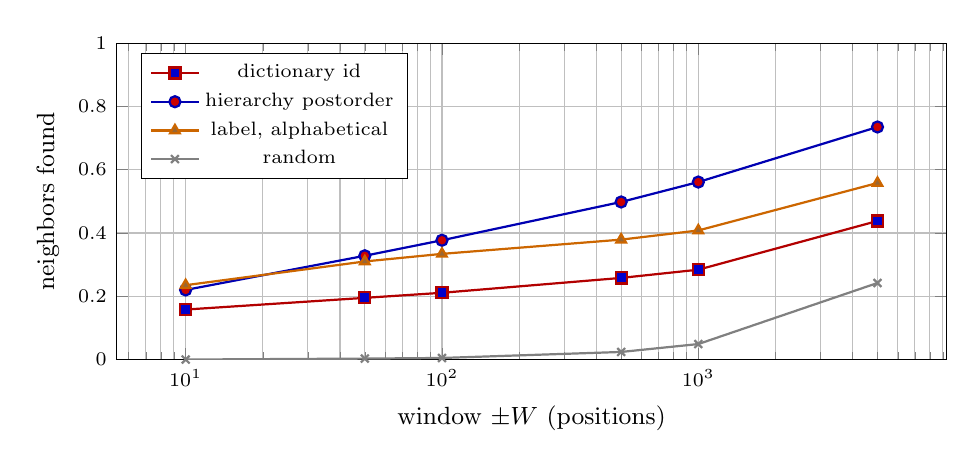
\begin{tikzpicture}
\begin{axis}[width=\columnwidth,height=5.6cm,xmode=log,xlabel={window $\pm W$ (positions)},ylabel={neighbors found},ymin=0,ymax=1,grid=both,legend pos=north west,legend style={font=\scriptsize},tick label style={font=\scriptsize},label style={font=\small}]
\addplot+[mark=square*,color=red!70!black,thick] coordinates {(10,0.158) (50,0.195) (100,0.211) (500,0.258) (1000,0.284) (5000,0.438)};
\addlegendentry{dictionary id}
\addplot+[mark=*,color=blue!70!black,thick] coordinates {(10,0.22) (50,0.328) (100,0.377) (500,0.498) (1000,0.561) (5000,0.735)};
\addlegendentry{hierarchy postorder}
\addplot+[mark=triangle*,color=orange!80!black,thick] coordinates {(10,0.235) (50,0.31) (100,0.334) (500,0.379) (1000,0.408) (5000,0.558)};
\addlegendentry{label, alphabetical}
\addplot+[mark=x,color=gray,thick] coordinates {(10,0) (50,0.003) (100,0.005) (500,0.024) (1000,0.049) (5000,0.242)};
\addlegendentry{random}
\end{axis}
\end{tikzpicture}

\caption{The data of Table~\ref{tab-order}: the share of neighbors found within $\pm W$ positions, by order.}
\label{fig-order}
\end{figure}

Three things follow.
First, the postorder of the class hierarchy is the best order, and much better
than first-seen ids: the nearest neighbor is 45 positions away instead of
1,739.
Second, even so, a scan of 100 positions finds 38\% of the ten neighbors, and
a window of $\pm$1,000 positions (2.6\% of the ontology) still misses 44\%;
Lemma~\ref{lem-bw} is not an artifact of the grid.
Third, first-seen ids are not random: the ontology's ids were minted in related
batches, so ids carry some locality (0.21 at $\pm$100) that depends on the file
and not on the engine.
Of the ten neighbors, 12\% are a parent or child and 32\% are within two
\texttt{is\_a} steps, while a two-step neighborhood holds only 45 terms
(0.12\% of the ontology), so hierarchy proximity is highly informative about
meaning without being sufficient.
The order is therefore useful for structure and not a substitute for a vector
index.

\section{Hierarchies as Intervals}
\label{sec-labels}

An instance query $\mathrm{inst}(c)$ (Definition~\ref{def-queries}) must return
the instances of every class in $\desc(c)$.
A store can \emph{materialize} the entailed type triples, or \emph{rewrite}
the query into one scan per class in $\desc(c)$.
\sys instead numbers the classes so that $\desc(c)$ is a few integer
intervals, and keeps the numbers in the B+ tree it already has.

\stitle{Labelling}.
Collapse each cycle of $H$ into one class.
Choose a spanning forest by taking, for each class with several parents, the
parent with the longest path from a root.
Number the classes $1,\dots,|\mathcal{C}|$ in postorder of the forest, and let
$\lo(c)$ be the smallest number in the forest subtree of $c$.
In a forest, $u\in\desc(c)$ if and only if $\lo(c)\le\po(u)\le\po(c)$, a
single interval.
In a DAG each class carries a \emph{set} of intervals $I(c)$, built bottom-up
(Algorithm~\ref{alg-label}).

\begin{algorithm}[t]
\caption{Interval sets for a class DAG}\label{alg-label}
\small
\KwIn{subclass edges $E$ of $H$}
\KwOut{$\po(c)$ and an interval set $I(c)$ for each class $c$}
collapse the strongly connected components of $H$ (Tarjan), and number them parents first\;
\For{each component $c$, parents first}{
  $\mathit{depth}(c) \gets 1 + \max_{c'}\ \mathit{depth}(c')$ over its parents $c'$ \tcp*{0 for a root}
  $\mathit{tp}(c) \gets$ the parent with the largest depth\;
}
number the forest $\{(c,\mathit{tp}(c))\}$ in postorder; record $\lo(c)$\;
\For{each component $c$, children first}{
  $I(c) \gets \textsc{Merge}\big(\{[\lo(c),\po(c)]\} \cup \bigcup_{c'\text{ a child of }c} I(c')\big)$ \tcp*{sort; join overlapping or adjacent}
}
\end{algorithm}

\begin{lemma}[Correctness]\label{lem-correct}
$u\in\desc(c)$ if and only if $\po(u)$ lies in an interval of $I(c)$.
\end{lemma}
\iffull
\begin{proof}
By induction over the order in which Algorithm~\ref{alg-label} builds $I$: the
numbers covered by $I(c)$ are exactly those of the classes in $\desc(c)$.
\end{proof}
\fi

\begin{lemma}[Size]\label{lem-size}
For every class $c$, $|I(c)|\le 1+|E'(c)|$, where $E'(c)$ is the set of non-tree edges whose tail is in $\desc(c)$.
\end{lemma}
\iffull
\begin{proof}
A class $u\in\desc(c)$ is reached from $c$ by a path.
If the path uses no non-tree edge, $u$ is in the forest subtree of $c$.
Otherwise let $\epsilon$ be the last non-tree edge on it; $u$ is then in the forest
subtree of the head of $\epsilon$.
So the covered set is the forest subtree of $c$ together with the forest
subtrees of the heads of the edges of $E'(c)$, a union of $1+|E'(c)|$
intervals.
\end{proof}
\fi

The labelling takes $O(|\mathcal{C}|+|E|)$ plus the merges, and a tree needs
one interval per class.

\stitle{Index}.
The labels go into B+ trees of \sys: key $(\po(c),\mathit{id}(c),0)$ for each
class, and $(\po(c),\mathit{id}(e),0)$ for each triple $(e,\texttt{rdf:type},c)$.
The classes below $c$, or the instances of $c$ and its subclasses, are then
one range scan $[\,(a,0,0),\,(b{+}1,0,0)\,)$ per interval $[a,b]$ of $I(c)$,
and the answers of different intervals are disjoint.
Inserting an instance adds one key; deleting a class edge rebuilds the labels,
which takes tens of milliseconds for an ontology of tens of thousands of
classes.
Incremental maintenance with gaps in the numbering~\cite{agrawal1989} is not
implemented.
Dictionary ids are untouched: ids appear in three permutations, the log, and
checkpoints, and renumbering them to follow the hierarchy would rewrite all of
it.
The label tree is separate and rebuildable, which keeps ids stable.

\stitle{Membership}.
A class $u$ is below $c$ if $\po(u)$ lies in an interval of $I(c)$, a binary
search over $|I(c)|$ intervals with no scan.
This makes the class filter of Section~\ref{sec-vectors} a constant-space
predicate on a term's number.

\section{Entailment-Aware Query Planning}
\label{sec-rewrite}

The interval index answers the instance query $\mathrm{inst}(c)$ of
Section~\ref{sec-pre}, but a \sparql user writes \texttt{?x rdf:type $c$} and
receives the stored triples only: ten of the fourteen LUBM queries return no
rows (Section~\ref{sec-exp}).
\sys therefore offers RDFS subclass entailment as a \emph{plan rewrite}.
With \texttt{\textbackslash set entail on}, a type pattern with a constant
class is answered by the interval index, and the optimizer, the joins, and
every other operator are unchanged.

\stitle{Semantics}.
Let $\mathcal{T}^{+}$ be $\mathcal{T}$ together with $(e,\texttt{rdf:type},c')$ for
every $(e,\texttt{rdf:type},c)\in\mathcal{T}$ and every $c'$ with $c\in\desc(c')$.
A triple pattern $(s,\texttt{rdf:type},c)$ with a constant class has as
\emph{entailed answers} its answers over $\mathcal{T}^{+}$; every other pattern
is evaluated over $\mathcal{T}$.
A pattern whose class is a variable, a class the hierarchy does not contain,
and every other predicate are left as they were.
Only \texttt{rdfs:subClassOf} is read: no \texttt{rdfs:subPropertyOf}, domain,
range, or OWL axiom, and no inference over the properties of a query.

\stitle{The rewrite}.
Algorithm~\ref{alg-rewrite} runs on the planner's tree before the optimizer.
It replaces a qualifying scan by an \emph{interval type scan} and records how
many rows it expects, which is the number of type triples whose class label
lies in an interval of $I(c)$, read from prefix sums over the labels in
$O(|I(c)|)$ time.
The optimizer then orders the joins with that estimate, as it does for any
scan.
This matters: from the stored triples alone, \texttt{?x rdf:type Student}
looks empty, and a plan that starts from it starts from a pattern that in fact
returns 75,547 rows.

\begin{example}
Over \texttt{Dog}, \texttt{Cat} $\sqsubseteq$ \texttt{Mammal} $\sqsubseteq$ \texttt{Animal}
and \texttt{Bird} $\sqsubseteq$ \texttt{Animal}, the query
\texttt{SELECT ?x ?n WHERE \{ ?x a ex:Animal . ?x ex:name ?n \}} returns one row
without entailment (the entity typed \texttt{Animal} itself) and four with it.
\texttt{\textbackslash explain} shows the rewritten plan, in which the optimizer
has joined the interval scan to the name scan by index nested loops:
\begin{small}\begin{verbatim}
Projection [?x, ?n]
  IndexNestedLoopJoin
    IntervalTypeScan {?x rdf:type ex:Animal}
    TripleScan {?x ex:name ?n}
\end{verbatim}\end{small}
\end{example}

\begin{algorithm}[t]
\caption{\textsc{RewriteTypeScans}$(\mathit{plan})$}\label{alg-rewrite}
\small
\ForEach{triple-scan leaf $(s,p,o)$ of $\mathit{plan}$}{
  \If{$p$ is the constant \texttt{rdf:type}, $o$ is a constant class $c$ of the hierarchy $H$}{
    mark the scan as an interval type scan of $c$\;
    $\mathit{rows} \gets \sum_{[a,b]\in I(c)} \big(\mathit{cnt}(b)-\mathit{cnt}(a-1)\big)$ \tcp*{prefix sums of type triples by label}
  }
}
\end{algorithm}

\stitle{Execution}.
An interval type scan is still a scan: it yields triples
$(e,\texttt{rdf:type},c)$ for the instances of $c$, and the operators above
it read them as they read stored ones.
With a free subject it takes one range scan of the label tree per interval of
$I(c)$ and returns the distinct instances in ascending order.
With a bound subject, as when an index nested-loop join probes it with each
outer row, it reads the subject's stored types from the SPO tree and tests
each label against $I(c)$ by binary search.
An entailed triple is not stored, so a scan under a transaction locks the
triple set and not the triple.

\begin{lemma}[Soundness and completeness]\label{lem-rewrite}
For every class $c$ of the hierarchy, the interval type scan of $c$ returns
$(e,\texttt{rdf:type},c)$ if and only if this triple belongs to $\mathcal{T}^{+}$.
\end{lemma}
\iffull
\begin{proof}
The triple is in $\mathcal{T}^{+}$ iff $e$ has a stored type $c''$ with
$c''\in\desc(c)$.
The label tree holds $(\po(c''),e)$ for every stored type of every entity, so by
Lemma~\ref{lem-correct} $e$ is returned by the range scans of $I(c)$ iff
$\po(c'')$ lies in an interval of $I(c)$ for some stored type $c''$, that is,
iff $c''\in\desc(c)$.
A bound subject is tested with the same condition on its stored types.
\end{proof}
\fi

\stitle{Freshness}.
The hierarchy and the label tree are a snapshot, kept on a private file of the
same buffer-pool engine.
Every update, load, and backend switch advances a version number, and the first
entailed query after a change rebuilds the snapshot from the store: 0.06\,s
for LUBM(10) and its 43 classes, a few tens of milliseconds for the Gene
Ontology.
Incremental maintenance of the labels with gaps~\cite{agrawal1989} would avoid
the rebuild and is not implemented.
The snapshot is not part of a transaction, so an entailed query sees the
committed state at the time it built.

\section{Vector Indexes and Filtered Search}
\label{sec-vectors}

\sys keeps one unit-length float vector $\mathbf{v}(t)$ per term in memory,
loaded from a checksummed file whose records name terms by spelling, so a
file survives a dictionary that numbers terms differently.
Embeddings come from outside; \sys stores and searches them.
Four index families are available, each a different trade between
exactness, memory, and build time.

\stitle{Flat}.
Score every vector: $O(Nd)$ and exact.
With 8-bit scalar quantization (one scale $\delta=\max_i|v_i|/127$ per vector, for coordinates $v_i$) each
coordinate is off by at most $\delta/2$, so for a unit query a score is off by at
most $(\delta/2)\sqrt d$, in a quarter of the memory.

\stitle{IVF}.
Spherical $k$-means with $k$-means++ seeding~\cite{arthur2007} gives $\nu$
centroids and each vector goes to its nearest.
A query scores the centroids and reads the $\rho$ nearest lists.
The cost is $\nu d+\rho (N/\nu) d$, minimal at $\nu=\sqrt{\rho N}$.
The design choice is where the lists live: \emph{as key ranges of the B+ tree
that holds the triples}.
The pair (list, row) is a key $(\mathrm{list},\mathrm{row},0)$, so a list is a
prefix scan, an insert is a tree insert, and the lists page, cache, and latch
like every other index of the engine.
Under a filter the search keeps probing the nearest remaining lists until it
holds $k$ allowed rows, so a filter that excludes everything near the query
costs more instead of returning nothing.

\stitle{Product quantization (PQ)}.
Cut a vector into $m$ pieces and replace each by the index of its nearest of
256 learned centers~\cite{jegou2011}: $m$ bytes per vector.
A query builds $m$ tables of 256 dot products and scores a code as the sum of
$m$ lookups, which equals the dot product with the decoded vector, so all the
error is on the stored side.

\stitle{HNSW}.
The layered proximity graph of Malkov and Yashunin~\cite{malkov2020} with the
paper's neighbor-selection heuristic: a candidate is kept only if it is
nearer the new node than to every neighbor already kept.
Layer 0 allows $2M$ links, and the search beam is $\ef$.
Search takes an optional predicate and still crosses nodes it may not return.

\subsection{Filtering a Similarity Query by a Class}
\label{sec-hybrid}

A filtered similarity query $\mathrm{near}(q,c,k)$ asks for the $k$ terms of
$\desc(c)$ nearest to $q$.
Let $f(c)=|\desc(c)|/N$.
We compare four ways to answer it, all returning terms of $\desc(c)$ only.
\begin{description}
\item[Pre-filter.] Resolve $c$ to its members first (one range scan per
  interval of $I(c)$), then score only those, exactly. About $f(c)\,N\,d$ work.
\item[Post-filter.] Ask the index for $k'>k$ terms, keep those below $c$ (a
  membership test is a binary search over $I(c)$), and multiply $k'$ by four
  until $k$ remain or the index is exhausted.
  If the filter were independent of the similarity, about $k/f(c)$
  candidates would be needed.
\item[Masked search.] Give the index a predicate, ``the row's number lies in
  an interval of $I(c)$'', so a list scan or a graph walk skips rows outside
  $c$.
  Nothing is resolved in advance: each row the search touches costs one
  binary search.
  HNSW still crosses rows it may not return, to keep the graph connected, in
  the spirit of ACORN~\cite{patel2024}; IVF keeps probing lists until it has
  $k$ allowed rows.
\item[Auto.] Pre-filter when $|\desc(c)|$ is at most 4,096, otherwise masked
  HNSW.
\end{description}

\stitle{The filter is correlated with the vectors}.
In an ontology the names of a class's descendants are close to the class and
to each other, so the neighbors of a term tend to lie under the term's own
ancestors.
On the Gene Ontology, of the unfiltered top 100 neighbors of a query from
\emph{inside} $c$, 4\% to 72\% lie under $c$, rising with the size of $c$; for
a query from \emph{outside} $c$ the share is 0\% to 12\%.
The independence estimate $k/f(c)$ is therefore wrong in both directions:
post-filtering is cheap for an inside query and does not terminate usefully
for an outside one.

\stitle{Do not resolve the filter}.
A masked search that first resolved $c$ by interval scans and built a bitmap
per query spent most of its time resolving: for a class of over 5,000 members
that was 560 of 669 $\mu$s.
Testing the number of each row the search touches, one binary search over a
handful of intervals, brought the same search to 105 $\mu$s.
This is where interval labels earn their keep a second time: they make
membership an $O(\log|I(c)|)$ test with no scan.

\section{A Build for the Browser}
\label{sec-system}

The engine compiles with Emscripten to a 0.85\,MB WebAssembly
module~\cite{haas2017} that runs the same indexed store, planner, optimizer,
and semantic extension in a web page.
Two parts of the native build do not carry over, and replacing them is the
whole port.

\stitle{No raptor}.
The native loader parses RDF/XML, Turtle, and N-Triples with the raptor C
library.
The web build uses a Turtle and N-Triples parser of about 500 lines of our own
(prefixes, \texttt{a}, \texttt{;} and \texttt{,}, blank-node property lists,
collections, long strings, escapes, language tags, datatypes, and numeric and
boolean literals), and a test checks that it yields the same triples as
raptor on the shipped data.
RDF/XML needs the native build.

\stitle{No threads}.
The native engine has a disk-scheduler thread, a deadlock detector, and a
worker per session.
In the module the scheduler executes each request inline, the detector is not
started, and a statement runs on the calling thread; there is one session, so
there is nothing to deadlock.
The buffer pool, the page file (held in the browser's memory file system), the
B+ trees, and the plans are unchanged, so the page counts of
Section~\ref{sec-exp} and the plans the engine prints are the native ones.

\stitle{Using it}.
The module exports three functions: execute a statement, run a query and
return JSON, and reset.
The playground page built on them offers the memory store and the B+ tree
store on a buffer pool, shows the buffer-pool hits and misses of each query,
and loads an 834-class slice of the Gene Ontology with its embeddings.
In a desktop browser, building the interval labels for the slice takes 3\,ms,
the instance query for \emph{cell death} (97 classes, one range scan) 0.3\,ms,
a filtered similarity query 0.8\,ms, and building the IVF and HNSW indexes
58 and 98\,ms.
Updates are saved as a journal in the page's local storage and replayed when
the page loads, which keeps a session across reloads but is not durability:
there is no write-ahead log or recovery in the web build.

\stitle{No GPU}.
We considered WebGPU for the dot products and did not use it.
A similarity query scores a few hundred vectors with HNSW, or at most a few
thousand exactly; in the module that is under a millisecond with 128-bit SIMD,
which the build enables, and moving the query to a GPU and back costs more
than that.

\section{Experimental Study}
\label{sec-exp}

We evaluate \sys along five research questions.
\begin{itemize}
\item \textbf{[RQ1] The store}: how does a B+ tree store with three
  permutations compare with an LSM-based, a Java B+ tree, and a relational
  store on triple patterns, queries, and loading?
\item \textbf{[RQ2] Hierarchies}: what do interval labels cost, and how do they
  compare with materializing and rewriting, and with other engines'
  subclass-path queries?
\item \textbf{[RQ3] Vector indexes}: what recall, time, and memory do the
  four indexes give on real embeddings?
\item \textbf{[RQ4] Filtered search}: which strategy answers
  $\mathrm{near}(q,c,k)$ fastest, and does a single rule choose well?
\item \textbf{[RQ5] Concurrency}: how do lookups and inserts scale with the
  number of threads, and what do readers see while a writer runs?
\item \textbf{[RQ6] Design choices}: what do three permutations, the bulk
  loader, and the decode cache each buy?
\end{itemize}

Table~\ref{tab-glance} summarizes the answers; the subsections give every
measurement.

\begin{table}[t]
\caption{Selected results: how many times faster \sys{} is than each other engine (the time of the other engine divided by \sys's; for throughput, \sys's divided by the other's). All tables of this section give every measurement.}
\label{tab-glance}
\small
\resizebox{\columnwidth}{!}{%
\begin{tabular}{@{}lrrrr@{}}
\toprule
 & Ox.\ RocksDB & Ox.\ memory & Jena TDB2 & SQLite \\
\midrule
pattern $(s,\cdot,\cdot)$ & 8.4$\times$ & 3.4$\times$ & 36.7$\times$ & 4.2$\times$ \\
pattern $(s,p,\cdot)$ & 7.2$\times$ & 4.6$\times$ & 27.3$\times$ & 5.5$\times$ \\
LUBM query 1 & 3.7$\times$ & 1.4$\times$ & 58.4$\times$ & 2.0$\times$ \\
instances of a class, 10--99 below & 39.1$\times$ & 7.7$\times$ & 47.9$\times$ & 14.9$\times$ \\
instances of a class, 1000+ below & 5.8$\times$ & 2.2$\times$ & 5.3$\times$ & 3.5$\times$ \\
lookups per second, 8 threads & 7.0$\times$ & 3.2$\times$ & 6.1$\times$ & 3.9$\times$ \\
lookups per second, 8 readers + 1 writer & 10.2$\times$ & 4.8$\times$ & 18.8$\times$ & 4.3$\times$ \\
\bottomrule
\end{tabular}}
\end{table}


\subsection{Experimental Setup}

\stitle{Systems}.
We compare \sys, built in release mode with the B+ tree store (SPO, POS, OSP),
a 256\,MiB buffer pool, and automatic join selection, with four configurations
of three other systems, all run in-process on one thread of the same
machine: Oxigraph 0.5.13~\cite{oxigraph} through its Rust interface, with
RocksDB on disk and with its in-memory store; Apache Jena TDB2
5.2.0~\cite{jenatdb} on Java 17 with a 4\,GiB heap and its own bulk loader;
and SQLite 3.51 with one table of three string columns, a primary key on
$(s,p,o)$ and two more indexes on $(p,o,s)$ and $(o,s,p)$, a SPARQL basic
graph pattern translated into a join of the table with itself, and
\texttt{ANALYZE} after loading.
SQLite stores terms as strings and \sys as ids; we include it as the
relational baseline.
RDF4J, QLever, and RDFox are discussed in Section~\ref{sec-related} but not run.
Concurrency is measured in-process: threads for \sys, Oxigraph, and Jena, and
processes with one connection each for SQLite, whose Python driver would
otherwise share one interpreter lock.

\stitle{Data}.
LUBM~\cite{lubm} at one and ten universities (103,104 and 1,316,700
statements) and the Gene Ontology~\cite{ashburner2000} (release 2026-07-26
without obsolete terms: 38,092 classes, 57,456 \texttt{is\_a} edges) with
$d=384$ embeddings of the term names by
\texttt{all-MiniLM-L6-v2}~\cite{reimers2019}.
Because the Gene Ontology has no instances, we add 200,000 synthetic
entities of one to three types drawn uniformly from its classes (495,552
triples in all).

\stitle{Workloads and method}.
The pattern workload samples, from each dataset, 100 constants for every
bound position of each shape of Table~\ref{tab-perms}, so that every shape is
measured; the LUBM workload is the 14 queries of the benchmark.
The instance workload asks for $\mathrm{inst}(c)$ for 30 classes in each of
five size buckets, answered by \sys through interval scans and by the others
through the subclass path \texttt{?c rdfs:subClassOf* c . ?x a ?c} (SQLite: a
recursive query).
Each query is parsed once, run to warm the caches (three times for the JVM and SQLite), and then five to nine times; we report the median, and the mean of
medians over a workload.
Every engine converts each answer to its string, and the row counts of all
engines agree on every query.
Queries that run for a minute are reported as timeouts; none did.
Times are warm: they include \sys's decode cache and the other engines' own
caches.
The machine is an Apple M2 Pro with 16\,GiB.
Counts of page reads use a cold 64-frame pool.
The code, data generators, and every number in this section are available
at the artifact URL.

\subsection{RQ1: The Store}

Table~\ref{tab-load} gives the cost of loading LUBM(10), and
Table~\ref{tab-queries} the query times.

\begin{table}[t]
\caption{Loading LUBM in each engine (bulk loader, one thread of the loader, files on a local SSD). Oxigraph's count is distinct triples; \sys's is statements read.}
\label{tab:load}
\small
\resizebox{\columnwidth}{!}{%
\begin{tabular}{@{}llrrrr@{}}
\toprule
Data & Engine & triples & load (s) & disk (MiB) & RSS (MiB) \\
\midrule
LUBM(1) & \sys{} & 103\,104 & 1.02 & 10.8 & 322 \\
 & Oxigraph, RocksDB & 100\,573 & 0.13 & 17.8 & 60 \\
 & Oxigraph, memory & 100\,573 & 0.18 & --- & 53 \\
\midrule
LUBM(10) & \sys{} & 1\,316\,700 & 13.83 & 133.7 & 637 \\
 & Oxigraph, RocksDB & 1\,272\,953 & 1.95 & 176.3 & 87 \\
 & Oxigraph, memory & 1\,272\,953 & 2.32 & --- & 546 \\
\bottomrule
\end{tabular}}
\end{table}


\begin{table*}[t]
\caption{Query times on LUBM(10): the mean over 100 sampled constants per pattern shape (all 18 predicates for $(\cdot,p,\cdot)$), and the median of the four LUBM queries that return rows without inference. Row counts agree across engines.}
\label{tab-queries}
\small
\begin{tabular}{@{}lrrrrrr@{}}
\toprule
Query & rows & \sys{} & Ox.\ RocksDB & Ox.\ memory & Jena TDB2 & SQLite \\
\midrule
$(s,\cdot,\cdot)$ & 7 & 3\,$\mu$s & 27\,$\mu$s & 11\,$\mu$s & 117\,$\mu$s & 13\,$\mu$s \\
$(s,p,\cdot)$ & 2 & 2\,$\mu$s & 14\,$\mu$s & 9\,$\mu$s & 52\,$\mu$s & 11\,$\mu$s \\
$(\cdot,\cdot,o)$ & 16,233 & 11.0\,ms & 35.7\,ms & 10.4\,ms & 23.7\,ms & 8.4\,ms \\
$(\cdot,p,o)$ & 16,225 & 10.2\,ms & 19.4\,ms & 7.8\,ms & 24.8\,ms & 6.2\,ms \\
$(\cdot,p,\cdot)$ & 70,720 & 70.8\,ms & 161.2\,ms & 41.2\,ms & 107.5\,ms & 35.5\,ms \\
\midrule
LUBM 1 & 4 & 9\,$\mu$s & 32\,$\mu$s & 12\,$\mu$s & 508\,$\mu$s & 18\,$\mu$s \\
LUBM 3 & 6 & 11\,$\mu$s & 37\,$\mu$s & 13\,$\mu$s & 234\,$\mu$s & 18\,$\mu$s \\
LUBM 2 (triangle) & 28 & 8.2\,ms & 275.1\,ms & 34.1\,ms & 120.1\,ms & 4.0\,ms \\
LUBM 14 (scan) & 75,547 & 46.0\,ms & 88.1\,ms & 40.8\,ms & 138.7\,ms & 29.3\,ms \\
\bottomrule
\end{tabular}
\end{table*}


\stitle{Selective patterns}.
For patterns that bind the subject, \sys takes 3\,$\mu$s and 2\,$\mu$s and the
others 11 to 117\,$\mu$s and 9 to 52\,$\mu$s: \sys is 3.4 to 37$\times$ faster
on $(s,\cdot,\cdot)$ and 4.6 to 27$\times$ on $(s,p,\cdot)$, and 1.4 to
58$\times$ faster on the selective LUBM queries.
Every answer is one descent of a B+ tree that fits the pool and a few keys.

\stitle{Large results}.
For patterns that return 16,000 to 71,000 rows, \sys takes 10 to 71\,ms: 1.9 to
3.2$\times$ faster than Oxigraph on RocksDB, 1.5 to 2.4$\times$ faster than
Jena, equal to Oxigraph's in-memory store on $(\cdot,\cdot,o)$ and 1.3 to
1.7$\times$ slower on the other two, and 1.3 to 2.0$\times$ slower than SQLite,
whose string index returns spellings without a dictionary.

\stitle{LUBM queries}.
Ten of the fourteen LUBM queries return no rows without inference; every
engine answers them in microseconds and the ratios of two tiny times mean
nothing, so Table~\ref{tab-queries} lists the four that return rows.
On the triangle query SQLite takes 4.0\,ms, \sys 8.2\,ms, Oxigraph in memory
34\,ms, Jena 120\,ms, and Oxigraph on RocksDB 275\,ms: \sys is 33$\times$
faster than the last, and twice as slow as SQLite; we did not inspect the
other engines' plans.
On the large scan (LUBM 14) the order is SQLite, Oxigraph in memory, \sys,
Oxigraph on RocksDB, Jena.

\stitle{Loading}.
\sys is the slowest to load, 11.4\,s against 2.0\,s for Oxigraph on RocksDB
(5.6$\times$), 6.1\,s for Jena, and 8.1\,s for SQLite, and its peak
memory is 584\,MiB against 78\,MiB for Oxigraph on RocksDB, because it
parses RDF/XML through a C library, interns each term through two B+ trees,
and builds exact statistics.
Its file is the smallest, 134\,MiB against 176 for Oxigraph on RocksDB, 363
for Jena, and 706 for SQLite.
In sum, a B+ tree store of three permutations is competitive with the
other designs on basic graph patterns: fastest on selective ones, within a
factor of two of the best on large ones, and slowest to load.

\subsection{RQ2: Hierarchies}

\stitle{Interval labels}.
Table~\ref{tab-labels} shows that the Gene Ontology needs 76,570 intervals for
38,092 classes, 2.01 per class and 598\,KiB in all, where the closure it
replaces has 393,448 ancestor pairs (9\,MiB as 24-byte keys in one
permutation).
The choice of spanning forest matters little: taking the deepest parent saves
13\%.
The tail is long, one class needing 741 intervals, within the bound of
Lemma~\ref{lem-size}.
Labels build in 15\,ms, and asking whether a class is below another takes
27\,ns against 775\,ns for a search up the parents.

\begin{table}[t]
\caption{Interval labels for the Gene Ontology.}
\label{tab-labels}
\small
\resizebox{\columnwidth}{!}{%
\begin{tabular}{@{}lrrrr@{}}
\toprule
Spanning-forest rule & non-tree edges & intervals & mean / p99 / max & build \\
\midrule
deepest parent & 19,367 & 76,570 & 2.01 / 17 / 741 & 14.9 ms \\
first parent & 19,367 & 87,769 & 2.30 / 22 / 740 & 14.4 ms \\
\bottomrule
\end{tabular}}
\end{table}

\stitle{Against materializing and rewriting}.
Table~\ref{tab-desc} compares interval scans with a search that scans POS once
per class.
For a class with a thousand or more descendants the intervals need 101
scans instead of 3,304, 40 page reads instead of 694, and 0.5\,ms instead of
9\,ms.
Table~\ref{tab-types} compares the three strategies for instance queries on
the synthetic instances.
Materializing the closure turns 495,552 triples into 4,017,973 (8.1$\times$),
the file from 63.6 to 309.5\,MiB, and the load from 5.1 to 180\,s.
The interval index adds 9.3\,MiB (15\%) and 0.17\,s.
On queries the interval index is close to the materialized store and far from
rewriting: for a class with a thousand or more descendants it reads 265 pages
against 182 (materialized) and 12,803 (rewrite).
All three return identical answers on every sampled class.
On LUBM(1) the hierarchy is shallow (43 classes) and the three are within a
factor of about two on every query, and materialization adds 15\% to the
triples: the benefit of intervals grows with the depth and breadth of the
hierarchy.

\begin{table}[t]
\caption{Descendants of a class in GO, cold 64-frame pool, mean over up to 40 classes per row.}
\label{tab-desc}
\small
\begin{tabular}{@{}lrrrr@{}}
\toprule
Below $c$ & method & scans & page reads & $\mu$s \\
\midrule
10--99 & intervals & 5.9 & 5.8 & 59 \\
 & one scan per class & 30.6 & 16.3 & 149 \\
100--999 & intervals & 29.1 & 13.2 & 147 \\
 & one scan per class & 268.2 & 65.7 & 803 \\
1000+ & intervals & 101.3 & 40.1 & 528 \\
 & one scan per class & 3303.6 & 694.1 & 8998 \\
\bottomrule
\end{tabular}
\end{table}

\begin{table}[t]
\caption{Instances of $c$ on 200,000 synthetic entities over GO, mean over 30 classes per row (cold 64-frame pool). Top: cost of the store.}
\label{tab-types}
\small
\begin{tabular}{@{}lrrr@{}}
\toprule
Strategy & triples & file (MiB) & load (s) \\
\midrule
rewrite & 495,552 & 63.6 & 5.09 \\
intervals & 495,552 & 72.9 & 5.26 \\
materialize & 4,017,973 & 309.5 & 180.31 \\
\bottomrule
\end{tabular}

\medskip
\begin{tabular}{@{}lrrrr@{}}
\toprule
Below $c$ & strategy & answers & page reads & $\mu$s \\
\midrule
10--99 & intervals & 278 & 8.4 & 90 \\
 & rewrite & 278 & 87.5 & 571 \\
 & materialized & 278 & 6.6 & 444 \\
100--999 & intervals & 2,954 & 40.9 & 1,461 \\
 & rewrite & 2,954 & 1,153 & 7,280 \\
 & materialized & 2,954 & 22.5 & 987 \\
1000+ & intervals & 29,904 & 264.8 & 4,555 \\
 & rewrite & 29,904 & 12,803 & 82,441 \\
 & materialized & 29,904 & 182.0 & 3,776 \\
\bottomrule
\end{tabular}
\end{table}

\stitle{Against other engines}.
Table~\ref{tab-hier} compares \sys with the other engines on instance
queries.
The interval scan alone returns term ids, in 1.9\,ms for the 29,904 answers of
the largest classes (about 60\,ns each); returning strings, as the others do, takes
11.5\,ms because each id is decoded.
At the string level \sys is 2.2$\times$ faster than the best other engine
(Oxigraph in memory) on the largest classes, 3.5$\times$ faster than SQLite's
recursive query, and 5.4 to 5.8$\times$ faster than Jena and Oxigraph on
RocksDB, and 5 to 9$\times$ faster than Oxigraph in memory on classes with
fewer than 1,000 instances.
With the decode cache off (Table~\ref{tab-cache}) \sys takes 22.6\,ms for the
largest classes, still 1.1$\times$ faster than the best other engine.
A subclass path is evaluated by the others as a graph traversal followed by a
join, and by \sys as range scans of one tree that return disjoint answers.

\begin{table}[t]
\caption{Instances of a class and its subclasses, 200\,000 entities over the Gene Ontology, 30 classes per row, warm: mean time. \sys{} answers by interval scans; Oxigraph by \texttt{?x a ?c . ?c rdfs:subClassOf* <C>}. \sys{} ``ids'' stops before the dictionary; ``strings'' decodes every answer, as Oxigraph does.}
\label{tab:hier}
\small
\resizebox{\columnwidth}{!}{%
\begin{tabular}{@{}lrrrrr@{}}
\toprule
Below $C$ & answers & \sys{} ids & \sys{} strings & Ox., RocksDB & Ox., memory \\
\midrule
1 & 10 & 1\,$\mu$s & 11\,$\mu$s & 37\,$\mu$s & 13\,$\mu$s \\
2-9 & 40 & 3\,$\mu$s & 42\,$\mu$s & 91\,$\mu$s & 23\,$\mu$s \\
10-99 & 278 & 10\,$\mu$s & 275\,$\mu$s & 539\,$\mu$s & 110\,$\mu$s \\
100-999 & 2,954 & 127\,$\mu$s & 2.9\,ms & 5.4\,ms & 1.1\,ms \\
1000+ & 29,904 & 1.7\,ms & 29.1\,ms & 60.6\,ms & 21.8\,ms \\
\bottomrule
\end{tabular}}
\end{table}


\subsection{RQ3: Vector Indexes}

We ran 1,000 query terms (the term itself excluded from its answer) against
all 38,092 vectors, with exact search as ground truth.
Table~\ref{tab-knn} gives selected points and Figure~\ref{fig-knn} the
recall--latency curves.

\begin{table}[t]
\caption{Vector indexes on GO (recall@10, mean time per query, memory of the structure, build time).}
\label{tab-knn}
\small
\resizebox{\columnwidth}{!}{%
\begin{tabular}{@{}llrrrr@{}}
\toprule
Index & setting & recall & $\mu$s & MiB & build (s) \\
\midrule
flat float32 & exact & 1.000 & 2,238 & 55.8 & --- \\
flat 8-bit & exact over codes & 0.996 & 4,554 & 14.1 & --- \\
flat PQ $m{=}48$ & codes only & 0.778 & 819 & 1.7 & 10.4 \\
flat PQ $m{=}48$ & re-rank 100 & 0.998 & 905 & 1.7$^\dagger$ & 10.4 \\
IVF $\nu{=}512$ & $\rho{=}8$ & 0.892 & 149 & 56.5 & 17.5 \\
IVF $\nu{=}512$ & $\rho{=}16$ & 0.929 & 255 & 56.5 & 17.5 \\
IVF $\nu{=}512$ & $\rho{=}64$ & 0.976 & 928 & 56.5 & 17.5 \\
IVF $\nu{=}512$, 8-bit & $\rho{=}16$ & 0.926 & 263 & 14.8 & 17.5 \\
IVF $\nu{=}512$, PQ 96 & $\rho{=}16$ & 0.839 & 178 & 4.2 & 38.4 \\
HNSW $M{=}16$ & $\ef{=}10$ & 0.993 & 44 & 59.7 & 15.0 \\
HNSW $M{=}16$ & $\ef{=}40$ & 0.997 & 108 & 59.7 & 15.0 \\
HNSW $M{=}32$ & $\ef{=}160$ & 0.999 & 474 & 63.4 & 28.0 \\
\bottomrule
\end{tabular}}

\smallskip
{\footnotesize $^\dagger$ re-ranking reads the float vectors as well.}
\end{table}

\begin{figure}[t]
\centering
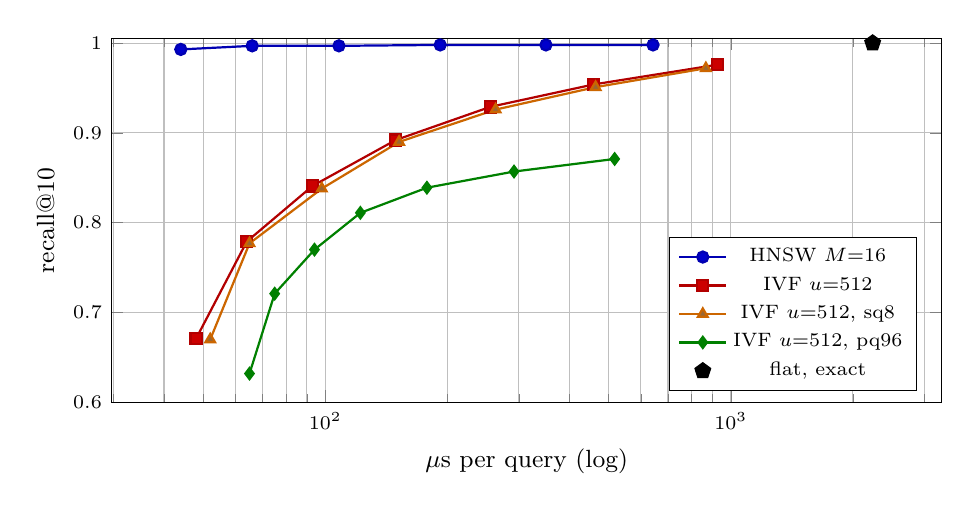
\begin{tikzpicture}
\begin{axis}[width=\columnwidth,height=6.2cm,xmode=log,xlabel={$\mu$s per query (log)},ylabel={recall@10},ymin=0.6,ymax=1.005,grid=both,legend pos=south east,legend style={font=\scriptsize},tick label style={font=\scriptsize},label style={font=\small}]
\addplot+[mark=*,color=blue!70!black,thick] coordinates {(44,0.993) (66,0.997) (108,0.997) (192,0.998) (350,0.998) (643,0.998)};
\addlegendentry{HNSW $M{=}16$}
\addplot+[mark=square*,color=red!70!black,thick] coordinates {(48,0.671) (64,0.779) (93,0.841) (149,0.892) (255,0.929) (459,0.954) (928,0.976)};
\addlegendentry{IVF $
u{=}512$}
\addplot+[mark=triangle*,color=orange!80!black,thick] coordinates {(52,0.67) (65,0.777) (98,0.838) (152,0.89) (263,0.926) (464,0.951) (868,0.972)};
\addlegendentry{IVF $
u{=}512$, sq8}
\addplot+[mark=diamond*,color=green!50!black,thick] coordinates {(65,0.632) (75,0.721) (94,0.77) (122,0.811) (178,0.839) (292,0.857) (517,0.871)};
\addlegendentry{IVF $
u{=}512$, pq96}
\addplot[only marks,mark=pentagon*,mark size=3pt,color=black] coordinates {(2238,1)};
\addlegendentry{flat, exact}
\end{axis}
\end{tikzpicture}

\caption{Recall@10 against time per query on GO (38,092 vectors, 384 dimensions).}
\label{fig-knn}
\end{figure}

\stitle{A baseline that is not slow by accident}.
Our first run scored with a plain dot-product loop.
A compiler may not vectorize it without \texttt{-ffast-math}, and the exact
scan took 8.3\,ms, which would have made the speed-ups look about twice as
large: HNSW at $\ef{=}10$ is 103 times faster than that baseline and 51 times
faster than the vectorized one.
With eight independent accumulators the exact scan takes 2.2\,ms (13
Gflop/s), and every number here uses that.
A speed-up over ``exact'' depends entirely on how fast exact is.

\stitle{What the numbers say}.
HNSW dominates on this data: recall 0.993 at 44\,$\mu$s, 51$\times$ faster
than the exact scan, for 3.9\,MiB of links on top of the vectors.
IVF needs 255\,$\mu$s for 0.929 and 928\,$\mu$s for 0.976.
IVF over the B+ tree is about 2.7$\times$ more expensive per scored row than a
contiguous scan (157\,ns against 59\,ns): each entry is a decoded 24-byte key
and a random read of the vector.
That is the price of lists that page, cache, and update with the triples.
The cost model holds in shape: more lists make a query cheaper until the
centroid scan dominates ($\nu{=}2048$ pays 124\,$\mu$s at $\rho{=}1$).
Product quantization is for memory, not speed, at this size: codes alone
reach 0.78 or 0.88 recall in 1.7 or 3.5\,MiB, and re-ranking the best 100
exactly recovers 0.998 and 1.000 but needs the float vectors.
8-bit codes keep 0.996 recall in a quarter of the memory and are slower than
float32, because converting bytes to floats costs more than the cache misses
they avoid at 56\,MiB.
The queries are terms of the ontology, whose neighbors are also terms of it;
queries from outside the vocabulary, such as free text, would be harder, and
we do not measure them.

\subsection{RQ4: Filtered Search}

For 20 classes in each of five size buckets we ran the ten nearest terms
under $c$ for a query inside $c$ and one outside it, against the exact answer
over the members.
IVF uses 512 lists and 16 probes, HNSW $M{=}16$ and $\ef{=}64$.
Table~\ref{tab-hybrid} gives recall and time.

\begin{table*}[t]
\caption{Ten nearest terms under a class $c$, by subtree size, query inside or outside $c$: recall@10 / $\mu$s per query. GO, 38,092 terms. Masked and post-filtered searches use the index; pre-filter resolves the members and scores them exactly.}
\label{tab-hybrid}
\small
\begin{tabular}{@{}lccccc@{}}
\toprule
Strategy & $\le$10 & 11--100 & 101--1000 & 1001--5000 & $>$5000 \\
\midrule
\multicolumn{6}{@{}l}{\emph{query inside $c$}} \\
pre-filter & 1.00 / 3 & 1.00 / 9 & 1.00 / 62 & 1.00 / 292 & 1.00 / 1,404 \\
post-filter, HNSW & 1.00 / 37,553 & 1.00 / 1,739 & 1.00 / 427 & 1.00 / 70 & 1.00 / 68 \\
post-filter, IVF & 0.86 / 903 & 0.87 / 558 & 0.93 / 293 & 0.98 / 198 & 0.99 / 211 \\
masked HNSW & 1.00 / 16,653 & 1.00 / 15,846 & 1.00 / 1,150 & 1.00 / 183 & 1.00 / 105 \\
masked IVF & 1.00 / 1,253 & 0.95 / 111 & 0.96 / 104 & 0.98 / 124 & 0.99 / 161 \\
auto & 1.00 / 3 & 1.00 / 9 & 1.00 / 59 & 1.00 / 269 & 1.00 / 95 \\
\midrule
\multicolumn{6}{@{}l}{\emph{query outside $c$}} \\
pre-filter & 1.00 / 3 & 1.00 / 9 & 1.00 / 62 & 1.00 / 291 & 1.00 / 1,394 \\
post-filter, HNSW & 1.00 / 36,654 & 1.00 / 27,669 & 0.99 / 13,607 & 1.00 / 5,513 & 1.00 / 836 \\
post-filter, IVF & 0.07 / 966 & 0.02 / 1,009 & 0.17 / 902 & 0.33 / 811 & 0.64 / 591 \\
masked HNSW & 1.00 / 16,802 & 1.00 / 16,611 & 1.00 / 8,697 & 1.00 / 4,424 & 1.00 / 900 \\
masked IVF & 1.00 / 1,255 & 0.79 / 698 & 0.45 / 286 & 0.37 / 147 & 0.66 / 107 \\
auto & 1.00 / 3 & 1.00 / 9 & 1.00 / 62 & 1.00 / 295 & 1.00 / 860 \\
\bottomrule
\end{tabular}
\end{table*}

\stitle{Exact pre-filtering wins for small classes}.
Up to about 1,000 members, resolving the members through the interval index
and scoring them exactly takes 3 to 62\,$\mu$s and is the exact answer.
Every index-based strategy is slower, from 1.7$\times$ (masked IVF at 101 to
1,000 members, at recall 0.96) to over 10,000$\times$ (post-filtered HNSW on
the smallest classes), because few of the vectors an index touches belong to
the class.
A graph search for a rare filter crosses most of the graph: masked HNSW reads
16\,ms for a class of at most 100 members, the failure ACORN is designed to
remove.

\stitle{Post-filtering fails for outside queries}.
IVF post-filter recall falls to 0.07 on the smallest classes and 0.64 on the
largest; HNSW reaches full recall only by searching again and again (37\,ms
for a class of at most ten members, in six rounds).

\stitle{Masked HNSW wins for large classes}.
Above 5,000 members it takes 105\,$\mu$s inside and 900\,$\mu$s outside,
exact, against 1.4\,ms for resolving and scoring the members.

\stitle{A cost model for the crossover}.
Let $\gamma_m$ be the cost of pre-filtering per member (an interval scan, a hash
lookup from term to row, and one dot product); from Table~\ref{tab-hybrid},
$\gamma_m\approx 0.13$ to $0.20\,\mu$s for classes of a few hundred members or
more.
Pre-filtering beats a masked graph search when $|\desc(c)|<\theta=\gamma_h/\gamma_m$, where
$\gamma_h$ is the masked search's time.
For a query inside $c$, $\gamma_h\approx 105$ to $183\,\mu$s, so $\theta\approx 800$ to
1,000, which matches the observed crossing between the 101--1,000 and
1,001--5,000 columns.
For a query outside $c$ the masked walk costs 0.9 to 4.4\,ms on classes of
1,000 or more members, so $\theta$ is 7,000 to 25,000.
A single threshold has to sit between the two; 4,096 stays below the
outside-query crossing and loses at most a factor of 3.8 at the inside-query
one.

\stitle{The auto rule}.
With a threshold of 4,096 members, auto matches the fastest strategy in every
cell but one and is never slower than 0.9\,ms.
The exception is a class of 1,001 to 5,000 members with an inside query:
269\,$\mu$s, against 70\,$\mu$s for post-filtered HNSW and 183\,$\mu$s for
masked HNSW.
Post-filtering would cost 5.5\,ms for an outside query on the same class, so
the rule gives up a factor of 3.8 in one cell to avoid a factor of 79 in its
neighbor.

\subsection{RQ5: Concurrency}

We load LUBM(10) and run, for three seconds each, one to eight threads of
lookups (the $(s,\cdot,\cdot)$ and $(s,p,\cdot)$ queries, 200 in rotation),
one to eight threads of inserts of new triples with scattered subjects, and
one writer beside one to eight readers.
Figure~\ref{fig-conc} plots the lookups and Table~\ref{tab-conc} the rest.

\begin{figure}[t]
\centering
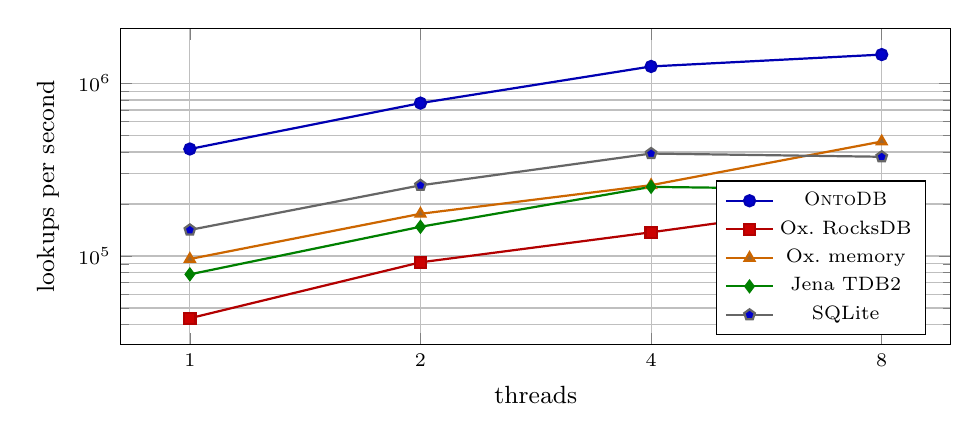
\begin{tikzpicture}
\begin{axis}[width=\columnwidth,height=5.6cm,xmode=log,ymode=log,log basis x=2,xtick={1,2,4,8},xticklabels={1,2,4,8},xlabel={threads},ylabel={lookups per second},grid=both,legend pos=south east,legend style={font=\scriptsize},tick label style={font=\scriptsize},label style={font=\small}]
\addplot+[mark=*,color=blue!70!black,thick] coordinates {(1,416050) (2,767222) (4,1250348) (8,1464779)};
\addlegendentry{\sys{}}
\addplot+[mark=square*,color=red!70!black,thick] coordinates {(1,43594) (2,91866) (4,137110) (8,208977)};
\addlegendentry{Ox.\ RocksDB}
\addplot+[mark=triangle*,color=orange!80!black,thick] coordinates {(1,96048) (2,175432) (4,256917) (8,459776)};
\addlegendentry{Ox.\ memory}
\addplot+[mark=diamond*,color=green!50!black,thick] coordinates {(1,78280) (2,147564) (4,251154) (8,241599)};
\addlegendentry{Jena TDB2}
\addplot+[mark=pentagon*,color=black!60,thick] coordinates {(1,141488) (2,256339) (4,391720) (8,375194)};
\addlegendentry{SQLite}
\end{axis}
\end{tikzpicture}

\caption{Lookups per second on LUBM(10) against the number of threads (both axes logarithmic).}
\label{fig-conc}
\end{figure}

\begin{table}[t]
\caption{Concurrency on LUBM(10): lookups per second with 1 and 8 reader threads, readers' lookups per second with one writer running, and inserts per second with 1 and 8 writer threads (one triple per transaction; \sys's inserts are not logged, and Jena's commit forces the journal to disk). The machine has 8 performance cores.}
\label{tab-conc}
\small
\resizebox{\columnwidth}{!}{%
\begin{tabular}{@{}lrrrrrr@{}}
\toprule
 & \multicolumn{2}{c}{lookups/s} & \multicolumn{2}{c}{readers + 1 writer} & \multicolumn{2}{c}{inserts/s} \\
\cmidrule(lr){2-3}\cmidrule(lr){4-5}\cmidrule(lr){6-7}
Engine & 1 & 8 & 1 & 8 & 1 & 8 \\
\midrule
\sys{} & 416k & 1.46M & 398k & 1.39M & 264k & 950k \\
Ox.\ RocksDB & 44k & 209k & 38k & 136k & 91k & 105k \\
Ox.\ memory & 96k & 460k & 69k & 288k & 679k & 186k \\
Jena TDB2 & 78k & 242k & 22k & 74k & 16 & 15 \\
SQLite & 141k & 375k & 111k & 322k & 15k & 14k \\
\bottomrule
\end{tabular}}
\end{table}


\stitle{Readers}.
\sys serves 416 thousand lookups per second with one thread and 1.46 million
with eight, 3.5 times more, and its single thread already beats every other
engine at eight threads except Oxigraph's in-memory store, which reaches 460
thousand.
At eight threads \sys serves 7.0, 3.2, 6.1, and 3.9 times the lookups of
Oxigraph on RocksDB, Oxigraph in memory, Jena TDB2, and SQLite.
Every engine scales with threads here; \sys's lead is its per-lookup cost, 2.4
microseconds, kept as threads are added.

\stitle{Readers beside a writer}.
With a writer inserting continuously, \sys's eight readers still serve 1.39
million lookups per second, 3.5 times its one-reader rate, while the writer
keeps inserting 111 thousand triples per second.
Beside a writer, eight readers reach 74 thousand lookups per second on Jena
TDB2, 136 thousand on Oxigraph on RocksDB, 288 thousand on Oxigraph in memory,
and 322 thousand on SQLite, so \sys's eight readers do 18.8, 10.2, 4.8, and 4.3
times as many.

\stitle{Writers}.
\sys's insert rate grows from 264 thousand per second with one thread to 950
thousand with eight, 3.6 times; Oxigraph on RocksDB gains 16\%, Oxigraph in
memory loses nearly three quarters, SQLite loses 4\%, and Jena TDB2's rate is bounded by
its commit.
The comparison favors \sys in one respect: its inserts here go through the
store without the write-ahead log, while the other engines commit each insert
with their default durability.
The scaling of \sys's own curve is the result; Oxigraph's in-memory store, which
is not durable either, inserts faster with one thread (679 thousand per
second).

\stitle{What limits it}.
Heavy queries scale less: the 16,000-row $(\cdot,p,o)$ query goes from 148 to 330
queries per second with eight threads, because it copies leaf after leaf and
decodes thousands of terms, so it is bound by memory traffic.
Splits and merges take the pessimistic path and serialize with each other on
the pages they share, and inserts into one leaf serialize on its latch.

\subsection{RQ6: Design Choices}

\stitle{Permutations}.
One tree, SPO, answers a pattern that does not bind the subject by a scan of
the whole tree.
Table~\ref{tab-permstudy} counts, on LUBM(1) with a cold 64-frame pool, the
page reads of a pattern for one, three, and all six permutations (averages
over 20 sampled patterns per shape).
Three permutations cut the pages of $(\cdot,p,\cdot)$ by 7.9$\times$ and those
of $(\cdot,\cdot,o)$ and $(\cdot,p,o)$ by 40$\times$; the other three trees
cost 66\% more space and change no pattern, because every shape already has
a prefix scan in the first three.

\begin{table}[t]
\caption{Page reads per pattern on LUBM(1) (cold 64-frame pool, bulk-loaded) and file size, by set of permutations.}
\label{tab-permstudy}
\small
\begin{tabular}{@{}lrrrr@{}}
\toprule
Permutations & $(\cdot,p,\cdot)$ & $(\cdot,\cdot,o)$ & $(\cdot,p,o)$ & file (MiB) \\
\midrule
SPO & 599 & 599 & 599 & 6.1 \\
SPO, POS, OSP & 76 & 15 & 15 & 10.8 \\
all six & 76 & 15 & 15 & 17.9 \\
\bottomrule
\end{tabular}
\end{table}

\stitle{Bulk loading}.
Loading the 15 files of LUBM(1) one triple at a time takes 1.74\,s and 16.2\,MiB
for three permutations; the bulk loader takes 1.08\,s and 10.8\,MiB, a third
less space, and a full scan reads 599 pages instead of 1,131 because
inserted leaves are about half full and bulk-loaded leaves are full.
With the loader, the time that remains is the dictionary's.

\stitle{Decode cache}.
Table~\ref{tab-cache} shows what the dictionary's decode cache buys:
the subject-bound pattern gets 4.3$\times$ faster, patterns that return
thousands of rows get 1.5 to 2.3$\times$ faster, and the largest instance
queries 2.0$\times$.
The cache does nothing for ids, which is why the
interval scan alone is 6$\times$ faster than the same query returning
strings.
A cache is the remedy Jena uses for the same cost; a cheaper id-to-spelling
access path would help every cold query and is future work.

\begin{table}[t]
\caption{The effect of \sys's decode cache (65\,536 entries) on the time to return strings: mean time per query on LUBM(10), and the instances of a class on the Gene Ontology (30 classes per row).}
\label{tab-cache}
\small
\begin{tabular}{@{}lrrr@{}}
\toprule
Workload & answers & cache off & cache on \\
\midrule
$(s,\cdot,\cdot)$ & 7 & 13\,$\mu$s & 3\,$\mu$s \\
$(s,p,\cdot)$ & 2 & 3\,$\mu$s & 2\,$\mu$s \\
$(\cdot,\cdot,o)$ & 16,233 & 24.9\,ms & 11.0\,ms \\
$(\cdot,p,o)$ & 16,225 & 14.9\,ms & 10.2\,ms \\
$(\cdot,p,\cdot)$ & 70,720 & 113.1\,ms & 70.8\,ms \\
\midrule
instances, 100-999 below & 2,954 & 2.4\,ms & 258\,$\mu$s \\
instances, 1000+ below & 29,904 & 22.6\,ms & 11.5\,ms \\
\bottomrule
\end{tabular}
\end{table}


\section{Related Work}
\label{sec-related}

\stitle{RDF stores}.
Triple stores keep triples in sorted permutations.
Hexastore indexes all six~\cite{weiss2008}; RDF-3X keeps six compressed B+
trees and prunes joins with statistics~\cite{neumann2010}; QLever builds
read-mostly permutation indexes in bulk~\cite{bast2017}; HDT is a compressed
read-only format~\cite{fernandez2013}; Virtuoso stores quads in a relational
engine~\cite{erling2010}.
Among systems we could run side by side, Apache Jena TDB2 uses B+
trees~\cite{jenatdb}, RDF4J's native store uses B-trees~\cite{rdf4j}, and
Oxigraph~\cite{oxigraph} keeps its indexes in RocksDB, a log-structured merge
tree.
\sys follows the B+ tree line with three permutations, which
Section~\ref{sec-exp} shows suffice.
The B+ tree~\cite{bayer1972,comer1979} and its concurrency and recovery
machinery~\cite{lehman1981,graefe2011,mohan1992} are textbook; the
contribution here is the choice of parts, their measured behavior on
ontologies, and what is built on top (Table~\ref{tab-related}).

\begin{table}[t]
\caption{Stores for ontologies, as documented (October 2026). We ran \sys, Oxigraph, Jena TDB2, and SQLite.}
\label{tab-related}
\small
\resizebox{\columnwidth}{!}{%
\begin{tabular}{@{}llll@{}}
\toprule
System & Triples are kept in & Hierarchy by & In a browser \\
\midrule
Oxigraph~\cite{oxigraph} & RocksDB (LSM) & query only & in-memory \\
Jena TDB2~\cite{jenatdb} & B+ trees & reasoner layer & no \\
RDF4J native~\cite{rdf4j} & B-trees & materialized & no \\
RDF-3X~\cite{neumann2010} & 6 compressed B+ trees & query only & no \\
RDFox~\cite{rdfox} & in memory & materialized & no \\
\sys & 3 B+ trees & intervals & full engine \\
\bottomrule
\end{tabular}}
\end{table}

\stitle{Inference}.
RDFS entailment is usually either \emph{rewritten} into the query or
\emph{materialized} at write time, with maintenance by counting or by
delete-and-rederive~\cite{gupta1993}.
Section~\ref{sec-labels} adds a third option that stores no entailed triple.
Agrawal, Borgida, and Jagadish~\cite{agrawal1989} store a compressed
transitive closure by numbering a spanning forest in postorder and giving each
node a set of intervals; Grust~\cite{grust2002} numbers XML trees in pre- and
postorder so that axes become regions of a plane.
We use the former on class DAGs inside a B+ tree store and measure it against
the other two ways to answer a type query.

\stitle{Vector search}.
Approximate nearest neighbor search has three families that matter here:
inverted files and product quantization~\cite{jegou2011}, proximity graphs, of
which HNSW~\cite{malkov2020} is the standard, and disk-oriented graphs such as
DiskANN~\cite{subramanya2019}.
FAISS~\cite{johnson2021} packages the first two.
Pan, Wang, and Li survey vector database systems and the hybrid queries
(attribute plus vector) that are hard for them~\cite{pan2024}.
ACORN~\cite{patel2024} makes HNSW traverse only the nodes that pass a
predicate.
Neo4j offers an HNSW vector index queried from Cypher~\cite{neo4jvec}; Amazon
Neptune Analytics offers vector similarity over graph nodes~\cite{neptunevec};
Fluree provides inline similarity functions and HNSW indexes for
RDF~\cite{fluree}; GraphDB has had similarity indexes queried from \sparql
since version 8~\cite{graphdbsim}.
In the documentation we read, none turns the class hierarchy into
range-scannable intervals, in the engine that holds the triples, to restrict
a vector search.
Euclidean embeddings of names are what we use; hyperbolic
embeddings~\cite{nickel2017} represent hierarchies more faithfully and would
change the vectors, not the indexes.

\stitle{Adaptive radix trees}.
An ART~\cite{leis2013} orders keys by byte, so its range scan is a lexical
range scan, the same one-dimensional order as a B+ tree, and
Lemma~\ref{lem-bw} applies to it.
Giving its leaves sibling links is possible and awkward: path compression and
node growth never move a leaf, but lazy expansion does, so a link that
pointed at the old leaf points at an inner node, and concurrent inserts must
latch both neighbors.
The usual alternative is a stack-based iterator that climbs and descends
between leaves.
\sys's keys are three fixed-width integers, which leave an ART little to
compress, so the B+ tree stays; DuckDB persists an ART for its own
keys~\cite{duckdbart}.

\stitle{Databases in the browser}.
WebAssembly~\cite{haas2017} lets a C++ engine run in a page.
Oxigraph ships a JavaScript build with an in-memory store.
\sys compiles the whole engine, including the paged B+ trees, the buffer pool,
and the semantic extension, by replacing the two parts that need threads or a
native library (Section~\ref{sec-system}).

\section{Conclusion}
\label{sec-conclude}

An ontology store is asked for patterns, for hierarchies, and for meaning.
This paper described \sys, which answers all three inside one disk-based
engine.
A B+ tree store of three permutations, with crabbing insert and delete, a range
scan that holds no latch between rows, and a bulk loader that fills pages,
answers selective patterns faster than an LSM store, a Java B+ tree store, and a
relational store, and is within a factor of two of the best on large results.
Labelling the class DAG with interval sets turns ``everything under $c$'' into
a few range scans of the same tree, at 2.0 intervals per class on the Gene
Ontology and a fraction of the cost of materializing the closure, and makes
membership in a class's subtree a binary search, which a filtered vector search
needs.
A sorted index orders and does not say what is close in meaning, which the
bandwidth argument and the measurements agree on; exact pre-filtering through
the intervals is the right answer for classes up to about a thousand members
and a masked graph search for the largest.
The whole engine runs in a browser from a 0.85\,MB module.

\stitle{Limitations}.
\sys implements a \sparql subset without \texttt{OPTIONAL}, \texttt{UNION},
property paths, or aggregates, and a reasoner only for
\texttt{rdfs:subClassOf}; a user who needs the full language needs one of the
other systems we measured.
It is the slowest to load, single-threaded, and hungry for memory while
loading, because its optimizer's exact statistics sit in hash tables.
Decoding an id costs about 0.7\,$\mu$s and dominates large results, which the
decode cache hides on a warm store and does not remove.
Labels are rebuilt, not maintained, when the hierarchy changes.
The vectors come from one ontology and one small model that embeds names only,
the instances of the Gene Ontology are synthetic, vectors are held in memory,
and the semantic measurements are single-threaded.
Queries are terms of the ontology; free text would need an embedding model that
\sys does not link.
We did not find a vector index that makes the hierarchy order unnecessary:
neighbors by meaning and descendants are different sets (a third of a term's
ten nearest neighbors are within two \texttt{is\_a} steps, two thirds are
not), which is why the two are combined at query time and not at index time.


\bibliographystyle{ACM-Reference-Format}
\bibliography{refs}

\clearpage
\appendix
\section{Further Algorithms}
\label{apx-alg}

These are the remaining algorithms of Sections~\ref{sec-store} and~\ref{sec-conc}, in the notation of Table~\ref{tab-notation}.

\subsection{Choosing a tree for a pattern}

\begin{algorithm}[h]
\caption{\textsc{ScanFor}$(s,p,o)$: choose a tree for a triple pattern}\label{alg-pattern}
\small
\For{each permutation $\pi \in \{\mathrm{SPO},\mathrm{POS},\mathrm{OSP}\}$}{
  $\ell(\pi) \gets$ the number of leading positions of $\pi$ that the pattern binds\;
}
$\pi^* \gets \arg\max_\pi \ell(\pi)$ (the first on a tie)\;
$x \gets$ the bound values in the order of $\pi^*$, padded with zeros\;
\Return $\textsc{Begin}(\mathrm{tree}(\pi^*), x, \ell(\pi^*))$, keeping the triples that match the pattern\;
\end{algorithm}

\subsection{Range scan}

\begin{algorithm}[h]
\caption{\textsc{BeginRange}$(a,b)$, \textsc{Take}, and \textsc{Settle}}\label{alg-range}
\small
$P \gets \textsc{LeafFor}(a)$; $i \gets$ the first position in $P$ with key $\ge a$\;
$\textsc{Take}(P, i)$; $\textsc{Settle}()$\;
\medskip
\textbf{Take}$(P, i)$: $\mathit{buf} \gets \langle P.\text{keys}[j] : j \ge i,\ \text{key} < b\rangle$; $\mathit{pos} \gets 0$\;
\quad $\mathit{next} \gets$ nil if some key $\ge b$ was met, else $P.\text{next}$; release $P$ (latch and pin)\;
\textbf{Settle}$()$: \While{$\mathit{pos} \ge |\mathit{buf}|$}{
  \lIf{$\mathit{next}$ is nil}{become the end iterator; \Return}
  $\textsc{Take}(\text{fetch}(\mathit{next}), 0)$ \tcp*{one sibling link, no climb to the root}
}
\medskip
\textbf{Advance}: $\mathit{pos} \gets \mathit{pos}+1$; \textsc{Settle}()\;
\end{algorithm}

\subsection{Bulk load}

\begin{algorithm}[h]
\caption{\textsc{BulkLoad}$(X)$ for a sorted set $X$ of unique keys}\label{alg-bulk}
\small
cut $X$ into runs of $B$ keys; if the last run has fewer than $\lfloor B/2\rfloor$, it and the run before it share their keys evenly\;
write each run as a leaf and link it to the previous one; $\Lambda \gets$ the list of (first key, page id)\;
\While{$|\Lambda| > 1$}{
  cut $\Lambda$ into runs of $F{+}1$ children, again sharing the last two runs evenly if the last is too short\;
  write each run as an internal page whose separators are the first keys of children $2,3,\dots$; $\Lambda \gets$ the (first key, id) of the new pages\;
}
set the root in the header to the page of $\Lambda[0]$\;
\end{algorithm}

\subsection{The optimistic descent for writers}

\begin{algorithm}[h]
\caption{\textsc{TryLeafOnly}$(x,\mathit{op})$ for an insert or a delete}\label{alg-optimistic}
\small
read-latch the header; $P \gets$ the root; \lIf{the tree is empty or $P$ is a leaf}{\Return fail}
read-latch $P$; release the header\;
\While{true}{
  $P' \gets \textsc{ChildFor}(P,x)$; pin $P'$ and read its type\;
  \lIf{$P'$ is internal}{read-latch $P'$; release $P$; $P \gets P'$; \textbf{continue}}
  write-latch $P'$ (the leaf); release $P$\;
  \If{$\mathit{op}$ is insert and $x \in P'$ or $\mathit{op}$ is delete and $x \notin P'$}{\Return done (no change)}
  \lIf{$\mathit{op}$ is insert and $P'$ is full, or $\mathit{op}$ is delete and $|P'| \le \lfloor B/2\rfloor$}{\Return fail}
  insert or remove $x$ in $P'$; \Return done\;
}
\end{algorithm}

\subsection{The latch-free fetch of a resident page}

\begin{algorithm}[h]
\caption{\textsc{Fetch}$(\mathit{id})$ in a shard, and the claim that guards eviction}\label{alg-fetch}
\small
$\varphi \gets \textsc{IndexFind}(\mathit{id})$ \tcp*{atomic array, no latch}
\If{$\varphi \ne \bot$ and \textsc{TryPin}(frame $\varphi$)}{
  \lIf{frame $\varphi$ holds page $\mathit{id}$}{mark frame $\varphi$ referenced; \Return frame $\varphi$}
  unpin frame $\varphi$ \tcp*{the frame was refilled}
}
latch the shard\;
\lIf{page $\mathit{id}$ is in the page table}{pin and return its frame}
$\varphi \gets$ a free frame, or else a victim:\;
\quad fold the \emph{referenced} marks into the replacer; mark frames with pin count 0 evictable\;
\quad \Repeat{a victim is claimed}{ask the replacer for the victim $v$; \textsc{TryClaim}$(v)$: swap pin count $0 \to -1$}\;
\quad write $v$ back if dirty; \textsc{IndexErase}$(v)$; drop $v$ from the page table\;
read page $\mathit{id}$ into $\varphi$; set its pin count to 1; \textsc{IndexInsert}$(\mathit{id}, \varphi)$; release the shard\;
\Return frame $\varphi$\;
\end{algorithm}



\end{document}
